% v1: three explanatory concepts; schematic signals, no inferred latent geometry.
\documentclass[tikz,border=0pt]{standalone}
\usepackage{amsmath}
\usetikzlibrary{arrows.meta,calc}
\definecolor{hl}{HTML}{0092B5}
\tikzset{>=Latex,line width=.7pt, lab/.style={font=\small},
 fixed/.style={black!55},learn/.style={hl},
 blk/.style={draw,rounded corners=1pt,minimum width=13mm,minimum height=7mm}}
\begin{document}
\begin{tikzpicture}\useasboundingbox (0,0) rectangle (16,9);\fill[white] (0,0) rectangle (16,9);\fontsize{12}{14}\selectfont
\node[anchor=west,font=\large\bfseries] at (0.6,8.4) {1 / S1: give the added states a prediction task};
\node[anchor=west,font=\scriptsize,text width=14.8cm,align=left] at (0.6,0.38) {Schematic, normalised; 30 samples per window. State superscripts n suppressed. S1 alternates with V updates; its target is fixed within each S1 step.};
\draw[hl] plot[smooth] coordinates {(1.0000,6.5000) (1.2000,6.5703) (1.4000,6.6348) (1.6000,6.6887) (1.8000,6.7281) (2.0000,6.7510) (2.2000,6.7574) (2.4000,6.7490) (2.6000,6.7291) (2.8000,6.7022) (3.0000,6.6730) (3.2000,6.6459) (3.4000,6.6246) (3.6000,6.6113) (3.8000,6.6065) (4.0000,6.6091) (4.2000,6.6162) (4.4000,6.6241) (4.6000,6.6285) (4.8000,6.6252) (5.0000,6.6110) (5.2000,6.5839) (5.4000,6.5437) (5.6000,6.4919) (5.8000,6.4319) (6.0000,6.3684) (6.2000,6.3068) (6.4000,6.2527) (6.6000,6.2110) (6.8000,6.1855) (7.0000,6.1784) (7.2000,6.1897) (7.4000,6.2177) (7.6000,6.2588) (7.8000,6.3085) (8.0000,6.3614) (8.2000,6.4122) (8.4000,6.4567) (8.6000,6.4916) (8.8000,6.5155) (9.0000,6.5287) (9.2000,6.5334) (9.4000,6.5326) (9.6000,6.5306) (9.8000,6.5315) (10.0000,6.5389) (10.2000,6.5551) (10.4000,6.5812) (10.6000,6.6163) (10.8000,6.6577) (11.0000,6.7017) (11.2000,6.7432) (11.4000,6.7772) (11.6000,6.7990) (11.8000,6.8050) (12.0000,6.7932) (12.2000,6.7635) (12.4000,6.7175) (12.6000,6.6591) (12.8000,6.5929)};
\fill[hl] (1.0000,6.5000) circle (.025);
\fill[hl] (1.2000,6.5703) circle (.025);
\fill[hl] (1.4000,6.6348) circle (.025);
\fill[hl] (1.6000,6.6887) circle (.025);
\fill[hl] (1.8000,6.7281) circle (.025);
\fill[hl] (2.0000,6.7510) circle (.025);
\fill[hl] (2.2000,6.7574) circle (.025);
\fill[hl] (2.4000,6.7490) circle (.025);
\fill[hl] (2.6000,6.7291) circle (.025);
\fill[hl] (2.8000,6.7022) circle (.025);
\fill[hl] (3.0000,6.6730) circle (.025);
\fill[hl] (3.2000,6.6459) circle (.025);
\fill[hl] (3.4000,6.6246) circle (.025);
\fill[hl] (3.6000,6.6113) circle (.025);
\fill[hl] (3.8000,6.6065) circle (.025);
\fill[hl] (4.0000,6.6091) circle (.025);
\fill[hl] (4.2000,6.6162) circle (.025);
\fill[hl] (4.4000,6.6241) circle (.025);
\fill[hl] (4.6000,6.6285) circle (.025);
\fill[hl] (4.8000,6.6252) circle (.025);
\fill[hl] (5.0000,6.6110) circle (.025);
\fill[hl] (5.2000,6.5839) circle (.025);
\fill[hl] (5.4000,6.5437) circle (.025);
\fill[hl] (5.6000,6.4919) circle (.025);
\fill[hl] (5.8000,6.4319) circle (.025);
\fill[hl] (6.0000,6.3684) circle (.025);
\fill[hl] (6.2000,6.3068) circle (.025);
\fill[hl] (6.4000,6.2527) circle (.025);
\fill[hl] (6.6000,6.2110) circle (.025);
\fill[hl] (6.8000,6.1855) circle (.025);
\fill[hl] (7.0000,6.1784) circle (.025);
\fill[hl] (7.2000,6.1897) circle (.025);
\fill[hl] (7.4000,6.2177) circle (.025);
\fill[hl] (7.6000,6.2588) circle (.025);
\fill[hl] (7.8000,6.3085) circle (.025);
\fill[hl] (8.0000,6.3614) circle (.025);
\fill[hl] (8.2000,6.4122) circle (.025);
\fill[hl] (8.4000,6.4567) circle (.025);
\fill[hl] (8.6000,6.4916) circle (.025);
\fill[hl] (8.8000,6.5155) circle (.025);
\fill[hl] (9.0000,6.5287) circle (.025);
\fill[hl] (9.2000,6.5334) circle (.025);
\fill[hl] (9.4000,6.5326) circle (.025);
\fill[hl] (9.6000,6.5306) circle (.025);
\fill[hl] (9.8000,6.5315) circle (.025);
\fill[hl] (10.0000,6.5389) circle (.025);
\fill[hl] (10.2000,6.5551) circle (.025);
\fill[hl] (10.4000,6.5812) circle (.025);
\fill[hl] (10.6000,6.6163) circle (.025);
\fill[hl] (10.8000,6.6577) circle (.025);
\fill[hl] (11.0000,6.7017) circle (.025);
\fill[hl] (11.2000,6.7432) circle (.025);
\fill[hl] (11.4000,6.7772) circle (.025);
\fill[hl] (11.6000,6.7990) circle (.025);
\fill[hl] (11.8000,6.8050) circle (.025);
\fill[hl] (12.0000,6.7932) circle (.025);
\fill[hl] (12.2000,6.7635) circle (.025);
\fill[hl] (12.4000,6.7175) circle (.025);
\fill[hl] (12.6000,6.6591) circle (.025);
\fill[hl] (12.8000,6.5929) circle (.025);
\draw[->] (0.8,5.7) -- (13.5,5.7);
\draw[dotted] (7,5.8) -- (7,7.5);
\node[] at (7,5.4) {$\tau$};
\node[] at (13.8,6.65) {$y^{\rm n}_k$};
\draw[] (0.9,7.6) -- (6.8,7.6);
\node[font=\small] at (3.7,7.85) {$\chi_\tau:\ (u,y)_{\tau-30:\tau-1}$};
\node[hl] at (8,1.7) {$\chi_\tau=(u,y)_{\tau-30:\tau-1}$};
\end{tikzpicture}
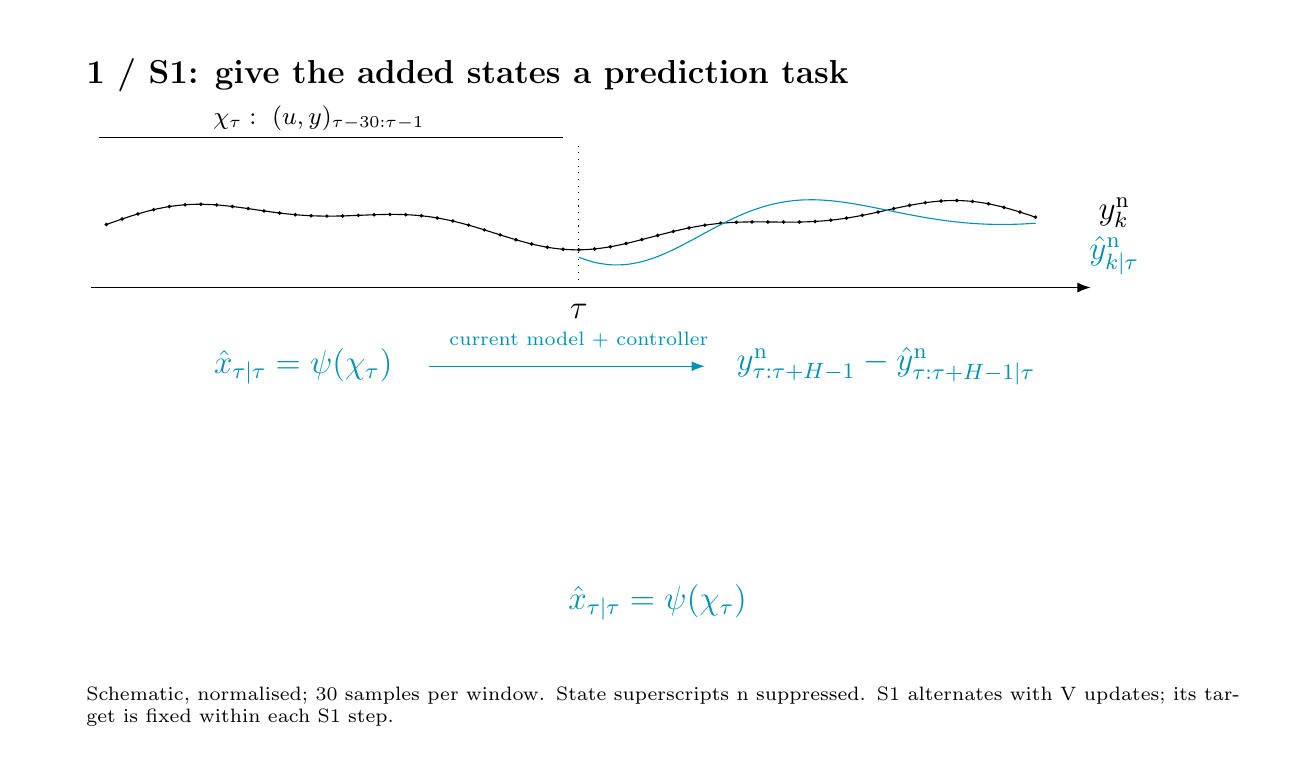
\begin{tikzpicture}\useasboundingbox (0,0) rectangle (16,9);\fill[white] (0,0) rectangle (16,9);\fontsize{12}{14}\selectfont
\node[anchor=west,font=\large\bfseries] at (0.6,8.4) {1 / S1: give the added states a prediction task};
\node[anchor=west,font=\scriptsize,text width=14.8cm,align=left] at (0.6,0.38) {Schematic, normalised; 30 samples per window. State superscripts n suppressed. S1 alternates with V updates; its target is fixed within each S1 step.};
\draw[black] plot[smooth] coordinates {(1.0000,6.5000) (1.2000,6.5703) (1.4000,6.6348) (1.6000,6.6887) (1.8000,6.7281) (2.0000,6.7510) (2.2000,6.7574) (2.4000,6.7490) (2.6000,6.7291) (2.8000,6.7022) (3.0000,6.6730) (3.2000,6.6459) (3.4000,6.6246) (3.6000,6.6113) (3.8000,6.6065) (4.0000,6.6091) (4.2000,6.6162) (4.4000,6.6241) (4.6000,6.6285) (4.8000,6.6252) (5.0000,6.6110) (5.2000,6.5839) (5.4000,6.5437) (5.6000,6.4919) (5.8000,6.4319) (6.0000,6.3684) (6.2000,6.3068) (6.4000,6.2527) (6.6000,6.2110) (6.8000,6.1855) (7.0000,6.1784) (7.2000,6.1897) (7.4000,6.2177) (7.6000,6.2588) (7.8000,6.3085) (8.0000,6.3614) (8.2000,6.4122) (8.4000,6.4567) (8.6000,6.4916) (8.8000,6.5155) (9.0000,6.5287) (9.2000,6.5334) (9.4000,6.5326) (9.6000,6.5306) (9.8000,6.5315) (10.0000,6.5389) (10.2000,6.5551) (10.4000,6.5812) (10.6000,6.6163) (10.8000,6.6577) (11.0000,6.7017) (11.2000,6.7432) (11.4000,6.7772) (11.6000,6.7990) (11.8000,6.8050) (12.0000,6.7932) (12.2000,6.7635) (12.4000,6.7175) (12.6000,6.6591) (12.8000,6.5929)};
\fill[black] (1.0000,6.5000) circle (.025);
\fill[black] (1.2000,6.5703) circle (.025);
\fill[black] (1.4000,6.6348) circle (.025);
\fill[black] (1.6000,6.6887) circle (.025);
\fill[black] (1.8000,6.7281) circle (.025);
\fill[black] (2.0000,6.7510) circle (.025);
\fill[black] (2.2000,6.7574) circle (.025);
\fill[black] (2.4000,6.7490) circle (.025);
\fill[black] (2.6000,6.7291) circle (.025);
\fill[black] (2.8000,6.7022) circle (.025);
\fill[black] (3.0000,6.6730) circle (.025);
\fill[black] (3.2000,6.6459) circle (.025);
\fill[black] (3.4000,6.6246) circle (.025);
\fill[black] (3.6000,6.6113) circle (.025);
\fill[black] (3.8000,6.6065) circle (.025);
\fill[black] (4.0000,6.6091) circle (.025);
\fill[black] (4.2000,6.6162) circle (.025);
\fill[black] (4.4000,6.6241) circle (.025);
\fill[black] (4.6000,6.6285) circle (.025);
\fill[black] (4.8000,6.6252) circle (.025);
\fill[black] (5.0000,6.6110) circle (.025);
\fill[black] (5.2000,6.5839) circle (.025);
\fill[black] (5.4000,6.5437) circle (.025);
\fill[black] (5.6000,6.4919) circle (.025);
\fill[black] (5.8000,6.4319) circle (.025);
\fill[black] (6.0000,6.3684) circle (.025);
\fill[black] (6.2000,6.3068) circle (.025);
\fill[black] (6.4000,6.2527) circle (.025);
\fill[black] (6.6000,6.2110) circle (.025);
\fill[black] (6.8000,6.1855) circle (.025);
\fill[black] (7.0000,6.1784) circle (.025);
\fill[black] (7.2000,6.1897) circle (.025);
\fill[black] (7.4000,6.2177) circle (.025);
\fill[black] (7.6000,6.2588) circle (.025);
\fill[black] (7.8000,6.3085) circle (.025);
\fill[black] (8.0000,6.3614) circle (.025);
\fill[black] (8.2000,6.4122) circle (.025);
\fill[black] (8.4000,6.4567) circle (.025);
\fill[black] (8.6000,6.4916) circle (.025);
\fill[black] (8.8000,6.5155) circle (.025);
\fill[black] (9.0000,6.5287) circle (.025);
\fill[black] (9.2000,6.5334) circle (.025);
\fill[black] (9.4000,6.5326) circle (.025);
\fill[black] (9.6000,6.5306) circle (.025);
\fill[black] (9.8000,6.5315) circle (.025);
\fill[black] (10.0000,6.5389) circle (.025);
\fill[black] (10.2000,6.5551) circle (.025);
\fill[black] (10.4000,6.5812) circle (.025);
\fill[black] (10.6000,6.6163) circle (.025);
\fill[black] (10.8000,6.6577) circle (.025);
\fill[black] (11.0000,6.7017) circle (.025);
\fill[black] (11.2000,6.7432) circle (.025);
\fill[black] (11.4000,6.7772) circle (.025);
\fill[black] (11.6000,6.7990) circle (.025);
\fill[black] (11.8000,6.8050) circle (.025);
\fill[black] (12.0000,6.7932) circle (.025);
\fill[black] (12.2000,6.7635) circle (.025);
\fill[black] (12.4000,6.7175) circle (.025);
\fill[black] (12.6000,6.6591) circle (.025);
\fill[black] (12.8000,6.5929) circle (.025);
\draw[->] (0.8,5.7) -- (13.5,5.7);
\draw[dotted] (7,5.8) -- (7,7.5);
\node[] at (7,5.4) {$\tau$};
\node[] at (13.8,6.65) {$y^{\rm n}_k$};
\draw[] (0.9,7.6) -- (6.8,7.6);
\node[font=\small] at (3.7,7.85) {$\chi_\tau:\ (u,y)_{\tau-30:\tau-1}$};
\draw[hl] plot[smooth] coordinates {(7.0000,6.0824) (7.2000,6.0195) (7.4000,5.9888) (7.6000,5.9923) (7.8000,6.0285) (8.0000,6.0935) (8.2000,6.1810) (8.4000,6.2832) (8.6000,6.3916) (8.8000,6.4982) (9.0000,6.5957) (9.2000,6.6785) (9.4000,6.7427) (9.6000,6.7864) (9.8000,6.8096) (10.0000,6.8140) (10.2000,6.8021) (10.4000,6.7775) (10.6000,6.7439) (10.8000,6.7051) (11.0000,6.6645) (11.2000,6.6248) (11.4000,6.5884) (11.6000,6.5571) (11.8000,6.5320) (12.0000,6.5141) (12.2000,6.5037) (12.4000,6.5009) (12.6000,6.5052) (12.8000,6.5160)};
\node[hl] at (13.8,6.1) {$\hat y^{\rm n}_{k|\tau}$};
\node[hl] at (3.5,4.7) {$\hat x_{\tau|\tau}=\psi(\chi_\tau)$};
\draw[hl,->] (5.1,4.7) -- (8.6,4.7);
\node[font=\scriptsize,hl] at (7,5.03) {current model + controller};
\node[hl] at (10.9,4.7) {$y^{\rm n}_{\tau:\tau+H-1}-\hat y^{\rm n}_{\tau:\tau+H-1|\tau}$};
\node[hl] at (8,1.7) {$\hat x_{\tau|\tau}=\psi(\chi_\tau)$};
\end{tikzpicture}
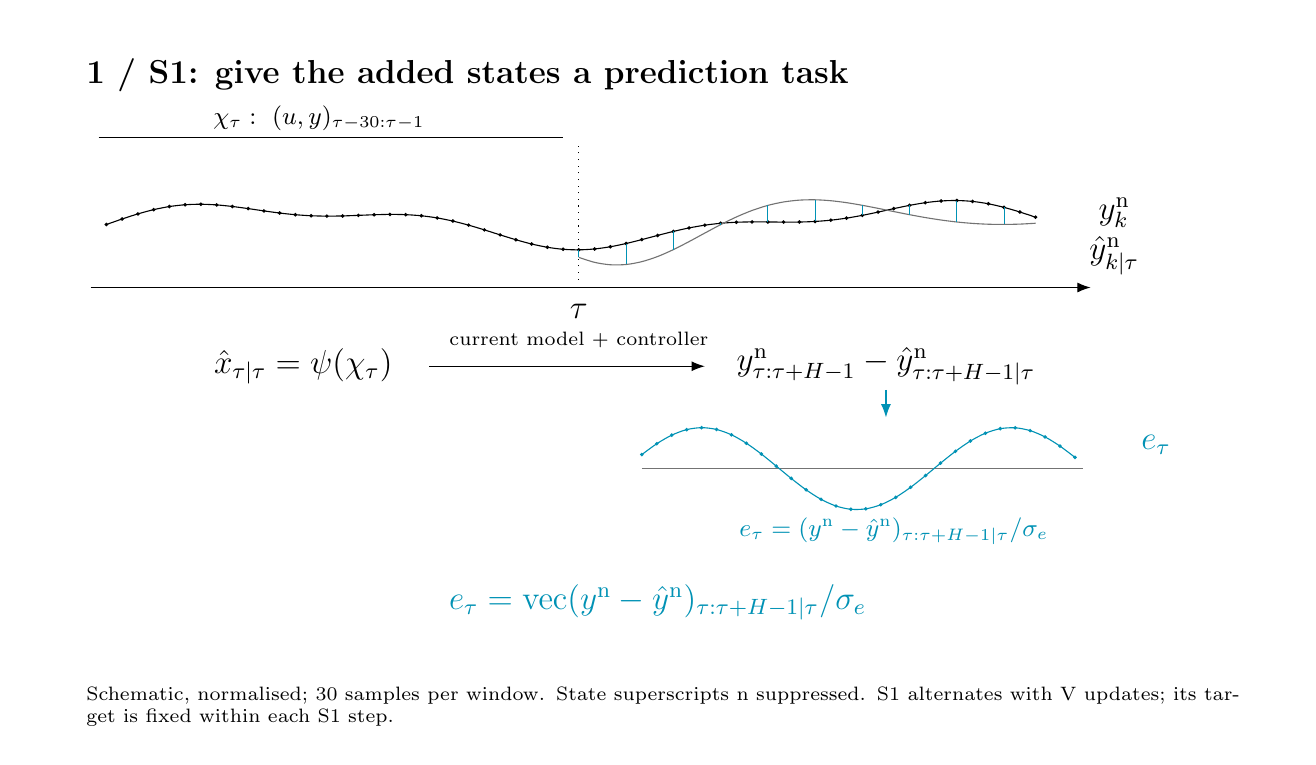
\begin{tikzpicture}\useasboundingbox (0,0) rectangle (16,9);\fill[white] (0,0) rectangle (16,9);\fontsize{12}{14}\selectfont
\node[anchor=west,font=\large\bfseries] at (0.6,8.4) {1 / S1: give the added states a prediction task};
\node[anchor=west,font=\scriptsize,text width=14.8cm,align=left] at (0.6,0.38) {Schematic, normalised; 30 samples per window. State superscripts n suppressed. S1 alternates with V updates; its target is fixed within each S1 step.};
\draw[black] plot[smooth] coordinates {(1.0000,6.5000) (1.2000,6.5703) (1.4000,6.6348) (1.6000,6.6887) (1.8000,6.7281) (2.0000,6.7510) (2.2000,6.7574) (2.4000,6.7490) (2.6000,6.7291) (2.8000,6.7022) (3.0000,6.6730) (3.2000,6.6459) (3.4000,6.6246) (3.6000,6.6113) (3.8000,6.6065) (4.0000,6.6091) (4.2000,6.6162) (4.4000,6.6241) (4.6000,6.6285) (4.8000,6.6252) (5.0000,6.6110) (5.2000,6.5839) (5.4000,6.5437) (5.6000,6.4919) (5.8000,6.4319) (6.0000,6.3684) (6.2000,6.3068) (6.4000,6.2527) (6.6000,6.2110) (6.8000,6.1855) (7.0000,6.1784) (7.2000,6.1897) (7.4000,6.2177) (7.6000,6.2588) (7.8000,6.3085) (8.0000,6.3614) (8.2000,6.4122) (8.4000,6.4567) (8.6000,6.4916) (8.8000,6.5155) (9.0000,6.5287) (9.2000,6.5334) (9.4000,6.5326) (9.6000,6.5306) (9.8000,6.5315) (10.0000,6.5389) (10.2000,6.5551) (10.4000,6.5812) (10.6000,6.6163) (10.8000,6.6577) (11.0000,6.7017) (11.2000,6.7432) (11.4000,6.7772) (11.6000,6.7990) (11.8000,6.8050) (12.0000,6.7932) (12.2000,6.7635) (12.4000,6.7175) (12.6000,6.6591) (12.8000,6.5929)};
\fill[black] (1.0000,6.5000) circle (.025);
\fill[black] (1.2000,6.5703) circle (.025);
\fill[black] (1.4000,6.6348) circle (.025);
\fill[black] (1.6000,6.6887) circle (.025);
\fill[black] (1.8000,6.7281) circle (.025);
\fill[black] (2.0000,6.7510) circle (.025);
\fill[black] (2.2000,6.7574) circle (.025);
\fill[black] (2.4000,6.7490) circle (.025);
\fill[black] (2.6000,6.7291) circle (.025);
\fill[black] (2.8000,6.7022) circle (.025);
\fill[black] (3.0000,6.6730) circle (.025);
\fill[black] (3.2000,6.6459) circle (.025);
\fill[black] (3.4000,6.6246) circle (.025);
\fill[black] (3.6000,6.6113) circle (.025);
\fill[black] (3.8000,6.6065) circle (.025);
\fill[black] (4.0000,6.6091) circle (.025);
\fill[black] (4.2000,6.6162) circle (.025);
\fill[black] (4.4000,6.6241) circle (.025);
\fill[black] (4.6000,6.6285) circle (.025);
\fill[black] (4.8000,6.6252) circle (.025);
\fill[black] (5.0000,6.6110) circle (.025);
\fill[black] (5.2000,6.5839) circle (.025);
\fill[black] (5.4000,6.5437) circle (.025);
\fill[black] (5.6000,6.4919) circle (.025);
\fill[black] (5.8000,6.4319) circle (.025);
\fill[black] (6.0000,6.3684) circle (.025);
\fill[black] (6.2000,6.3068) circle (.025);
\fill[black] (6.4000,6.2527) circle (.025);
\fill[black] (6.6000,6.2110) circle (.025);
\fill[black] (6.8000,6.1855) circle (.025);
\fill[black] (7.0000,6.1784) circle (.025);
\fill[black] (7.2000,6.1897) circle (.025);
\fill[black] (7.4000,6.2177) circle (.025);
\fill[black] (7.6000,6.2588) circle (.025);
\fill[black] (7.8000,6.3085) circle (.025);
\fill[black] (8.0000,6.3614) circle (.025);
\fill[black] (8.2000,6.4122) circle (.025);
\fill[black] (8.4000,6.4567) circle (.025);
\fill[black] (8.6000,6.4916) circle (.025);
\fill[black] (8.8000,6.5155) circle (.025);
\fill[black] (9.0000,6.5287) circle (.025);
\fill[black] (9.2000,6.5334) circle (.025);
\fill[black] (9.4000,6.5326) circle (.025);
\fill[black] (9.6000,6.5306) circle (.025);
\fill[black] (9.8000,6.5315) circle (.025);
\fill[black] (10.0000,6.5389) circle (.025);
\fill[black] (10.2000,6.5551) circle (.025);
\fill[black] (10.4000,6.5812) circle (.025);
\fill[black] (10.6000,6.6163) circle (.025);
\fill[black] (10.8000,6.6577) circle (.025);
\fill[black] (11.0000,6.7017) circle (.025);
\fill[black] (11.2000,6.7432) circle (.025);
\fill[black] (11.4000,6.7772) circle (.025);
\fill[black] (11.6000,6.7990) circle (.025);
\fill[black] (11.8000,6.8050) circle (.025);
\fill[black] (12.0000,6.7932) circle (.025);
\fill[black] (12.2000,6.7635) circle (.025);
\fill[black] (12.4000,6.7175) circle (.025);
\fill[black] (12.6000,6.6591) circle (.025);
\fill[black] (12.8000,6.5929) circle (.025);
\draw[->] (0.8,5.7) -- (13.5,5.7);
\draw[dotted] (7,5.8) -- (7,7.5);
\node[] at (7,5.4) {$\tau$};
\node[] at (13.8,6.65) {$y^{\rm n}_k$};
\draw[] (0.9,7.6) -- (6.8,7.6);
\node[font=\small] at (3.7,7.85) {$\chi_\tau:\ (u,y)_{\tau-30:\tau-1}$};
\draw[black!55] plot[smooth] coordinates {(7.0000,6.0824) (7.2000,6.0195) (7.4000,5.9888) (7.6000,5.9923) (7.8000,6.0285) (8.0000,6.0935) (8.2000,6.1810) (8.4000,6.2832) (8.6000,6.3916) (8.8000,6.4982) (9.0000,6.5957) (9.2000,6.6785) (9.4000,6.7427) (9.6000,6.7864) (9.8000,6.8096) (10.0000,6.8140) (10.2000,6.8021) (10.4000,6.7775) (10.6000,6.7439) (10.8000,6.7051) (11.0000,6.6645) (11.2000,6.6248) (11.4000,6.5884) (11.6000,6.5571) (11.8000,6.5320) (12.0000,6.5141) (12.2000,6.5037) (12.4000,6.5009) (12.6000,6.5052) (12.8000,6.5160)};
\node[black] at (13.8,6.1) {$\hat y^{\rm n}_{k|\tau}$};
\node[black] at (3.5,4.7) {$\hat x_{\tau|\tau}=\psi(\chi_\tau)$};
\draw[black,->] (5.1,4.7) -- (8.6,4.7);
\node[font=\scriptsize,black] at (7,5.03) {current model + controller};
\node[black] at (10.9,4.7) {$y^{\rm n}_{\tau:\tau+H-1}-\hat y^{\rm n}_{\tau:\tau+H-1|\tau}$};
\draw[hl] (7.0,6.1784) -- (7.0,6.0824);
\draw[hl] (7.6,6.2588) -- (7.6,5.9923);
\draw[hl] (8.2,6.4122) -- (8.2,6.181);
\draw[hl] (8.8,6.5155) -- (8.8,6.4982);
\draw[hl] (9.4,6.5326) -- (9.4,6.7427);
\draw[hl] (10.0,6.5389) -- (10.0,6.814);
\draw[hl] (10.6,6.6163) -- (10.6,6.7439);
\draw[hl] (11.2,6.7432) -- (11.2,6.6248);
\draw[hl] (11.8,6.805) -- (11.8,6.532);
\draw[hl] (12.4,6.7175) -- (12.4,6.5009);
\draw[black!55] (7.8,3.4) -- (13.4,3.4);
\draw[hl] plot[smooth] coordinates {(7.8000,3.5783) (7.9897,3.7161) (8.1793,3.8250) (8.3690,3.8951) (8.5586,3.9200) (8.7483,3.8974) (8.9379,3.8294) (9.1276,3.7222) (9.3172,3.5856) (9.5069,3.4320) (9.6966,3.2756) (9.8862,3.1304) (10.0759,3.0099) (10.2655,2.9250) (10.4552,2.8835) (10.6448,2.8891) (10.8345,2.9414) (11.0241,3.0355) (11.2138,3.1630) (11.4034,3.3120) (11.5931,3.4691) (11.7828,3.6199) (11.9724,3.7506) (12.1621,3.8493) (12.3517,3.9070) (12.5414,3.9184) (12.7310,3.8824) (12.9207,3.8024) (13.1103,3.6857) (13.3000,3.5429)};
\fill[hl] (7.8000,3.5783) circle (.025);
\fill[hl] (7.9897,3.7161) circle (.025);
\fill[hl] (8.1793,3.8250) circle (.025);
\fill[hl] (8.3690,3.8951) circle (.025);
\fill[hl] (8.5586,3.9200) circle (.025);
\fill[hl] (8.7483,3.8974) circle (.025);
\fill[hl] (8.9379,3.8294) circle (.025);
\fill[hl] (9.1276,3.7222) circle (.025);
\fill[hl] (9.3172,3.5856) circle (.025);
\fill[hl] (9.5069,3.4320) circle (.025);
\fill[hl] (9.6966,3.2756) circle (.025);
\fill[hl] (9.8862,3.1304) circle (.025);
\fill[hl] (10.0759,3.0099) circle (.025);
\fill[hl] (10.2655,2.9250) circle (.025);
\fill[hl] (10.4552,2.8835) circle (.025);
\fill[hl] (10.6448,2.8891) circle (.025);
\fill[hl] (10.8345,2.9414) circle (.025);
\fill[hl] (11.0241,3.0355) circle (.025);
\fill[hl] (11.2138,3.1630) circle (.025);
\fill[hl] (11.4034,3.3120) circle (.025);
\fill[hl] (11.5931,3.4691) circle (.025);
\fill[hl] (11.7828,3.6199) circle (.025);
\fill[hl] (11.9724,3.7506) circle (.025);
\fill[hl] (12.1621,3.8493) circle (.025);
\fill[hl] (12.3517,3.9070) circle (.025);
\fill[hl] (12.5414,3.9184) circle (.025);
\fill[hl] (12.7310,3.8824) circle (.025);
\fill[hl] (12.9207,3.8024) circle (.025);
\fill[hl] (13.1103,3.6857) circle (.025);
\fill[hl] (13.3000,3.5429) circle (.025);
\node[anchor=west,hl] at (14,3.7) {$e_\tau$};
\draw[->,hl] (10.9,4.4) -- (10.9,4.05);
\node[hl,font=\small] at (11,2.6) {$e_\tau=(y^{\rm n}-\hat y^{\rm n})_{\tau:\tau+H-1|\tau}/\sigma_e$};
\node[hl] at (8,1.7) {$e_\tau=\operatorname{vec}(y^{\rm n}-\hat y^{\rm n})_{\tau:\tau+H-1|\tau}/\sigma_e$};
\end{tikzpicture}
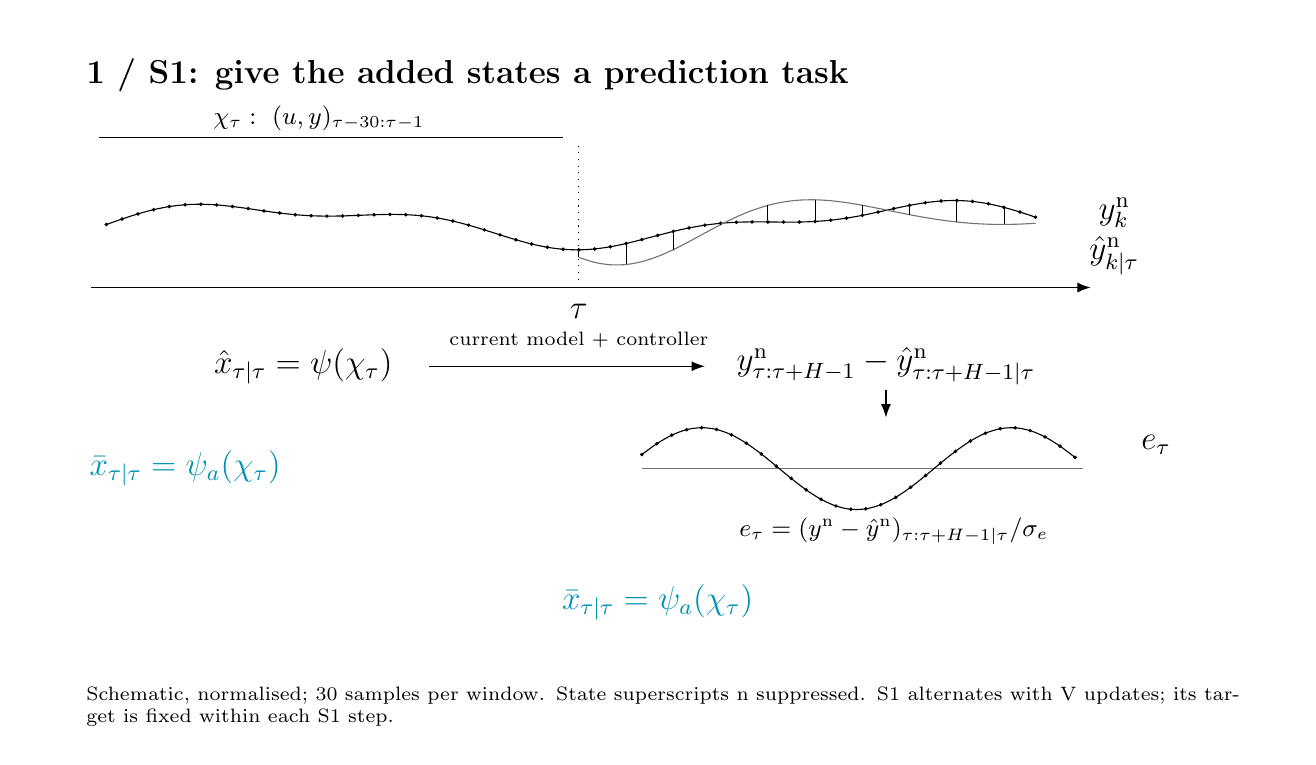
\begin{tikzpicture}\useasboundingbox (0,0) rectangle (16,9);\fill[white] (0,0) rectangle (16,9);\fontsize{12}{14}\selectfont
\node[anchor=west,font=\large\bfseries] at (0.6,8.4) {1 / S1: give the added states a prediction task};
\node[anchor=west,font=\scriptsize,text width=14.8cm,align=left] at (0.6,0.38) {Schematic, normalised; 30 samples per window. State superscripts n suppressed. S1 alternates with V updates; its target is fixed within each S1 step.};
\draw[black] plot[smooth] coordinates {(1.0000,6.5000) (1.2000,6.5703) (1.4000,6.6348) (1.6000,6.6887) (1.8000,6.7281) (2.0000,6.7510) (2.2000,6.7574) (2.4000,6.7490) (2.6000,6.7291) (2.8000,6.7022) (3.0000,6.6730) (3.2000,6.6459) (3.4000,6.6246) (3.6000,6.6113) (3.8000,6.6065) (4.0000,6.6091) (4.2000,6.6162) (4.4000,6.6241) (4.6000,6.6285) (4.8000,6.6252) (5.0000,6.6110) (5.2000,6.5839) (5.4000,6.5437) (5.6000,6.4919) (5.8000,6.4319) (6.0000,6.3684) (6.2000,6.3068) (6.4000,6.2527) (6.6000,6.2110) (6.8000,6.1855) (7.0000,6.1784) (7.2000,6.1897) (7.4000,6.2177) (7.6000,6.2588) (7.8000,6.3085) (8.0000,6.3614) (8.2000,6.4122) (8.4000,6.4567) (8.6000,6.4916) (8.8000,6.5155) (9.0000,6.5287) (9.2000,6.5334) (9.4000,6.5326) (9.6000,6.5306) (9.8000,6.5315) (10.0000,6.5389) (10.2000,6.5551) (10.4000,6.5812) (10.6000,6.6163) (10.8000,6.6577) (11.0000,6.7017) (11.2000,6.7432) (11.4000,6.7772) (11.6000,6.7990) (11.8000,6.8050) (12.0000,6.7932) (12.2000,6.7635) (12.4000,6.7175) (12.6000,6.6591) (12.8000,6.5929)};
\fill[black] (1.0000,6.5000) circle (.025);
\fill[black] (1.2000,6.5703) circle (.025);
\fill[black] (1.4000,6.6348) circle (.025);
\fill[black] (1.6000,6.6887) circle (.025);
\fill[black] (1.8000,6.7281) circle (.025);
\fill[black] (2.0000,6.7510) circle (.025);
\fill[black] (2.2000,6.7574) circle (.025);
\fill[black] (2.4000,6.7490) circle (.025);
\fill[black] (2.6000,6.7291) circle (.025);
\fill[black] (2.8000,6.7022) circle (.025);
\fill[black] (3.0000,6.6730) circle (.025);
\fill[black] (3.2000,6.6459) circle (.025);
\fill[black] (3.4000,6.6246) circle (.025);
\fill[black] (3.6000,6.6113) circle (.025);
\fill[black] (3.8000,6.6065) circle (.025);
\fill[black] (4.0000,6.6091) circle (.025);
\fill[black] (4.2000,6.6162) circle (.025);
\fill[black] (4.4000,6.6241) circle (.025);
\fill[black] (4.6000,6.6285) circle (.025);
\fill[black] (4.8000,6.6252) circle (.025);
\fill[black] (5.0000,6.6110) circle (.025);
\fill[black] (5.2000,6.5839) circle (.025);
\fill[black] (5.4000,6.5437) circle (.025);
\fill[black] (5.6000,6.4919) circle (.025);
\fill[black] (5.8000,6.4319) circle (.025);
\fill[black] (6.0000,6.3684) circle (.025);
\fill[black] (6.2000,6.3068) circle (.025);
\fill[black] (6.4000,6.2527) circle (.025);
\fill[black] (6.6000,6.2110) circle (.025);
\fill[black] (6.8000,6.1855) circle (.025);
\fill[black] (7.0000,6.1784) circle (.025);
\fill[black] (7.2000,6.1897) circle (.025);
\fill[black] (7.4000,6.2177) circle (.025);
\fill[black] (7.6000,6.2588) circle (.025);
\fill[black] (7.8000,6.3085) circle (.025);
\fill[black] (8.0000,6.3614) circle (.025);
\fill[black] (8.2000,6.4122) circle (.025);
\fill[black] (8.4000,6.4567) circle (.025);
\fill[black] (8.6000,6.4916) circle (.025);
\fill[black] (8.8000,6.5155) circle (.025);
\fill[black] (9.0000,6.5287) circle (.025);
\fill[black] (9.2000,6.5334) circle (.025);
\fill[black] (9.4000,6.5326) circle (.025);
\fill[black] (9.6000,6.5306) circle (.025);
\fill[black] (9.8000,6.5315) circle (.025);
\fill[black] (10.0000,6.5389) circle (.025);
\fill[black] (10.2000,6.5551) circle (.025);
\fill[black] (10.4000,6.5812) circle (.025);
\fill[black] (10.6000,6.6163) circle (.025);
\fill[black] (10.8000,6.6577) circle (.025);
\fill[black] (11.0000,6.7017) circle (.025);
\fill[black] (11.2000,6.7432) circle (.025);
\fill[black] (11.4000,6.7772) circle (.025);
\fill[black] (11.6000,6.7990) circle (.025);
\fill[black] (11.8000,6.8050) circle (.025);
\fill[black] (12.0000,6.7932) circle (.025);
\fill[black] (12.2000,6.7635) circle (.025);
\fill[black] (12.4000,6.7175) circle (.025);
\fill[black] (12.6000,6.6591) circle (.025);
\fill[black] (12.8000,6.5929) circle (.025);
\draw[->] (0.8,5.7) -- (13.5,5.7);
\draw[dotted] (7,5.8) -- (7,7.5);
\node[] at (7,5.4) {$\tau$};
\node[] at (13.8,6.65) {$y^{\rm n}_k$};
\draw[] (0.9,7.6) -- (6.8,7.6);
\node[font=\small] at (3.7,7.85) {$\chi_\tau:\ (u,y)_{\tau-30:\tau-1}$};
\draw[black!55] plot[smooth] coordinates {(7.0000,6.0824) (7.2000,6.0195) (7.4000,5.9888) (7.6000,5.9923) (7.8000,6.0285) (8.0000,6.0935) (8.2000,6.1810) (8.4000,6.2832) (8.6000,6.3916) (8.8000,6.4982) (9.0000,6.5957) (9.2000,6.6785) (9.4000,6.7427) (9.6000,6.7864) (9.8000,6.8096) (10.0000,6.8140) (10.2000,6.8021) (10.4000,6.7775) (10.6000,6.7439) (10.8000,6.7051) (11.0000,6.6645) (11.2000,6.6248) (11.4000,6.5884) (11.6000,6.5571) (11.8000,6.5320) (12.0000,6.5141) (12.2000,6.5037) (12.4000,6.5009) (12.6000,6.5052) (12.8000,6.5160)};
\node[black] at (13.8,6.1) {$\hat y^{\rm n}_{k|\tau}$};
\node[black] at (3.5,4.7) {$\hat x_{\tau|\tau}=\psi(\chi_\tau)$};
\draw[black,->] (5.1,4.7) -- (8.6,4.7);
\node[font=\scriptsize,black] at (7,5.03) {current model + controller};
\node[black] at (10.9,4.7) {$y^{\rm n}_{\tau:\tau+H-1}-\hat y^{\rm n}_{\tau:\tau+H-1|\tau}$};
\draw[black] (7.0,6.1784) -- (7.0,6.0824);
\draw[black] (7.6,6.2588) -- (7.6,5.9923);
\draw[black] (8.2,6.4122) -- (8.2,6.181);
\draw[black] (8.8,6.5155) -- (8.8,6.4982);
\draw[black] (9.4,6.5326) -- (9.4,6.7427);
\draw[black] (10.0,6.5389) -- (10.0,6.814);
\draw[black] (10.6,6.6163) -- (10.6,6.7439);
\draw[black] (11.2,6.7432) -- (11.2,6.6248);
\draw[black] (11.8,6.805) -- (11.8,6.532);
\draw[black] (12.4,6.7175) -- (12.4,6.5009);
\draw[black!55] (7.8,3.4) -- (13.4,3.4);
\draw[black] plot[smooth] coordinates {(7.8000,3.5783) (7.9897,3.7161) (8.1793,3.8250) (8.3690,3.8951) (8.5586,3.9200) (8.7483,3.8974) (8.9379,3.8294) (9.1276,3.7222) (9.3172,3.5856) (9.5069,3.4320) (9.6966,3.2756) (9.8862,3.1304) (10.0759,3.0099) (10.2655,2.9250) (10.4552,2.8835) (10.6448,2.8891) (10.8345,2.9414) (11.0241,3.0355) (11.2138,3.1630) (11.4034,3.3120) (11.5931,3.4691) (11.7828,3.6199) (11.9724,3.7506) (12.1621,3.8493) (12.3517,3.9070) (12.5414,3.9184) (12.7310,3.8824) (12.9207,3.8024) (13.1103,3.6857) (13.3000,3.5429)};
\fill[black] (7.8000,3.5783) circle (.025);
\fill[black] (7.9897,3.7161) circle (.025);
\fill[black] (8.1793,3.8250) circle (.025);
\fill[black] (8.3690,3.8951) circle (.025);
\fill[black] (8.5586,3.9200) circle (.025);
\fill[black] (8.7483,3.8974) circle (.025);
\fill[black] (8.9379,3.8294) circle (.025);
\fill[black] (9.1276,3.7222) circle (.025);
\fill[black] (9.3172,3.5856) circle (.025);
\fill[black] (9.5069,3.4320) circle (.025);
\fill[black] (9.6966,3.2756) circle (.025);
\fill[black] (9.8862,3.1304) circle (.025);
\fill[black] (10.0759,3.0099) circle (.025);
\fill[black] (10.2655,2.9250) circle (.025);
\fill[black] (10.4552,2.8835) circle (.025);
\fill[black] (10.6448,2.8891) circle (.025);
\fill[black] (10.8345,2.9414) circle (.025);
\fill[black] (11.0241,3.0355) circle (.025);
\fill[black] (11.2138,3.1630) circle (.025);
\fill[black] (11.4034,3.3120) circle (.025);
\fill[black] (11.5931,3.4691) circle (.025);
\fill[black] (11.7828,3.6199) circle (.025);
\fill[black] (11.9724,3.7506) circle (.025);
\fill[black] (12.1621,3.8493) circle (.025);
\fill[black] (12.3517,3.9070) circle (.025);
\fill[black] (12.5414,3.9184) circle (.025);
\fill[black] (12.7310,3.8824) circle (.025);
\fill[black] (12.9207,3.8024) circle (.025);
\fill[black] (13.1103,3.6857) circle (.025);
\fill[black] (13.3000,3.5429) circle (.025);
\node[anchor=west,black] at (14,3.7) {$e_\tau$};
\draw[->,black] (10.9,4.4) -- (10.9,4.05);
\node[black,font=\small] at (11,2.6) {$e_\tau=(y^{\rm n}-\hat y^{\rm n})_{\tau:\tau+H-1|\tau}/\sigma_e$};
\node[hl] at (2,3.4) {$\bar x_{\tau|\tau}=\psi_a(\chi_\tau)$};
\node[hl] at (8,1.7) {$\bar x_{\tau|\tau}=\psi_a(\chi_\tau)$};
\end{tikzpicture}
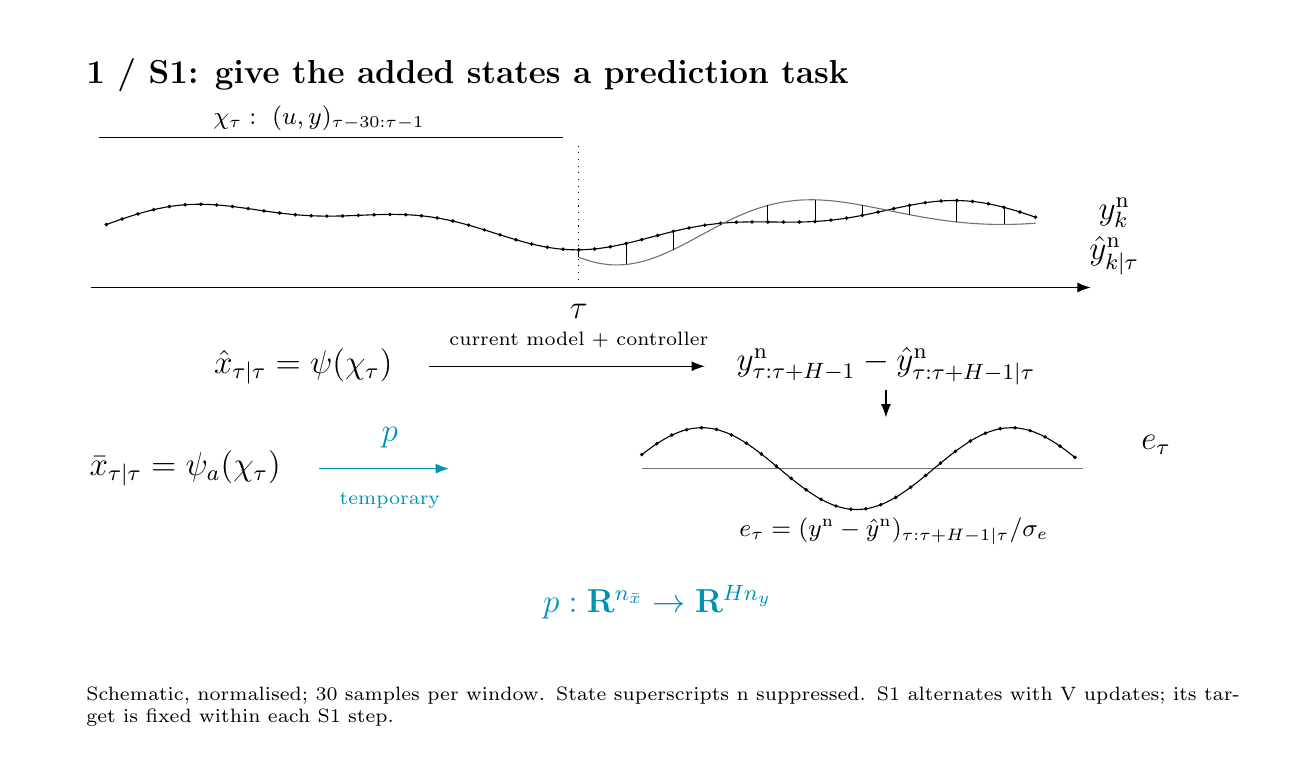
\begin{tikzpicture}\useasboundingbox (0,0) rectangle (16,9);\fill[white] (0,0) rectangle (16,9);\fontsize{12}{14}\selectfont
\node[anchor=west,font=\large\bfseries] at (0.6,8.4) {1 / S1: give the added states a prediction task};
\node[anchor=west,font=\scriptsize,text width=14.8cm,align=left] at (0.6,0.38) {Schematic, normalised; 30 samples per window. State superscripts n suppressed. S1 alternates with V updates; its target is fixed within each S1 step.};
\draw[black] plot[smooth] coordinates {(1.0000,6.5000) (1.2000,6.5703) (1.4000,6.6348) (1.6000,6.6887) (1.8000,6.7281) (2.0000,6.7510) (2.2000,6.7574) (2.4000,6.7490) (2.6000,6.7291) (2.8000,6.7022) (3.0000,6.6730) (3.2000,6.6459) (3.4000,6.6246) (3.6000,6.6113) (3.8000,6.6065) (4.0000,6.6091) (4.2000,6.6162) (4.4000,6.6241) (4.6000,6.6285) (4.8000,6.6252) (5.0000,6.6110) (5.2000,6.5839) (5.4000,6.5437) (5.6000,6.4919) (5.8000,6.4319) (6.0000,6.3684) (6.2000,6.3068) (6.4000,6.2527) (6.6000,6.2110) (6.8000,6.1855) (7.0000,6.1784) (7.2000,6.1897) (7.4000,6.2177) (7.6000,6.2588) (7.8000,6.3085) (8.0000,6.3614) (8.2000,6.4122) (8.4000,6.4567) (8.6000,6.4916) (8.8000,6.5155) (9.0000,6.5287) (9.2000,6.5334) (9.4000,6.5326) (9.6000,6.5306) (9.8000,6.5315) (10.0000,6.5389) (10.2000,6.5551) (10.4000,6.5812) (10.6000,6.6163) (10.8000,6.6577) (11.0000,6.7017) (11.2000,6.7432) (11.4000,6.7772) (11.6000,6.7990) (11.8000,6.8050) (12.0000,6.7932) (12.2000,6.7635) (12.4000,6.7175) (12.6000,6.6591) (12.8000,6.5929)};
\fill[black] (1.0000,6.5000) circle (.025);
\fill[black] (1.2000,6.5703) circle (.025);
\fill[black] (1.4000,6.6348) circle (.025);
\fill[black] (1.6000,6.6887) circle (.025);
\fill[black] (1.8000,6.7281) circle (.025);
\fill[black] (2.0000,6.7510) circle (.025);
\fill[black] (2.2000,6.7574) circle (.025);
\fill[black] (2.4000,6.7490) circle (.025);
\fill[black] (2.6000,6.7291) circle (.025);
\fill[black] (2.8000,6.7022) circle (.025);
\fill[black] (3.0000,6.6730) circle (.025);
\fill[black] (3.2000,6.6459) circle (.025);
\fill[black] (3.4000,6.6246) circle (.025);
\fill[black] (3.6000,6.6113) circle (.025);
\fill[black] (3.8000,6.6065) circle (.025);
\fill[black] (4.0000,6.6091) circle (.025);
\fill[black] (4.2000,6.6162) circle (.025);
\fill[black] (4.4000,6.6241) circle (.025);
\fill[black] (4.6000,6.6285) circle (.025);
\fill[black] (4.8000,6.6252) circle (.025);
\fill[black] (5.0000,6.6110) circle (.025);
\fill[black] (5.2000,6.5839) circle (.025);
\fill[black] (5.4000,6.5437) circle (.025);
\fill[black] (5.6000,6.4919) circle (.025);
\fill[black] (5.8000,6.4319) circle (.025);
\fill[black] (6.0000,6.3684) circle (.025);
\fill[black] (6.2000,6.3068) circle (.025);
\fill[black] (6.4000,6.2527) circle (.025);
\fill[black] (6.6000,6.2110) circle (.025);
\fill[black] (6.8000,6.1855) circle (.025);
\fill[black] (7.0000,6.1784) circle (.025);
\fill[black] (7.2000,6.1897) circle (.025);
\fill[black] (7.4000,6.2177) circle (.025);
\fill[black] (7.6000,6.2588) circle (.025);
\fill[black] (7.8000,6.3085) circle (.025);
\fill[black] (8.0000,6.3614) circle (.025);
\fill[black] (8.2000,6.4122) circle (.025);
\fill[black] (8.4000,6.4567) circle (.025);
\fill[black] (8.6000,6.4916) circle (.025);
\fill[black] (8.8000,6.5155) circle (.025);
\fill[black] (9.0000,6.5287) circle (.025);
\fill[black] (9.2000,6.5334) circle (.025);
\fill[black] (9.4000,6.5326) circle (.025);
\fill[black] (9.6000,6.5306) circle (.025);
\fill[black] (9.8000,6.5315) circle (.025);
\fill[black] (10.0000,6.5389) circle (.025);
\fill[black] (10.2000,6.5551) circle (.025);
\fill[black] (10.4000,6.5812) circle (.025);
\fill[black] (10.6000,6.6163) circle (.025);
\fill[black] (10.8000,6.6577) circle (.025);
\fill[black] (11.0000,6.7017) circle (.025);
\fill[black] (11.2000,6.7432) circle (.025);
\fill[black] (11.4000,6.7772) circle (.025);
\fill[black] (11.6000,6.7990) circle (.025);
\fill[black] (11.8000,6.8050) circle (.025);
\fill[black] (12.0000,6.7932) circle (.025);
\fill[black] (12.2000,6.7635) circle (.025);
\fill[black] (12.4000,6.7175) circle (.025);
\fill[black] (12.6000,6.6591) circle (.025);
\fill[black] (12.8000,6.5929) circle (.025);
\draw[->] (0.8,5.7) -- (13.5,5.7);
\draw[dotted] (7,5.8) -- (7,7.5);
\node[] at (7,5.4) {$\tau$};
\node[] at (13.8,6.65) {$y^{\rm n}_k$};
\draw[] (0.9,7.6) -- (6.8,7.6);
\node[font=\small] at (3.7,7.85) {$\chi_\tau:\ (u,y)_{\tau-30:\tau-1}$};
\draw[black!55] plot[smooth] coordinates {(7.0000,6.0824) (7.2000,6.0195) (7.4000,5.9888) (7.6000,5.9923) (7.8000,6.0285) (8.0000,6.0935) (8.2000,6.1810) (8.4000,6.2832) (8.6000,6.3916) (8.8000,6.4982) (9.0000,6.5957) (9.2000,6.6785) (9.4000,6.7427) (9.6000,6.7864) (9.8000,6.8096) (10.0000,6.8140) (10.2000,6.8021) (10.4000,6.7775) (10.6000,6.7439) (10.8000,6.7051) (11.0000,6.6645) (11.2000,6.6248) (11.4000,6.5884) (11.6000,6.5571) (11.8000,6.5320) (12.0000,6.5141) (12.2000,6.5037) (12.4000,6.5009) (12.6000,6.5052) (12.8000,6.5160)};
\node[black] at (13.8,6.1) {$\hat y^{\rm n}_{k|\tau}$};
\node[black] at (3.5,4.7) {$\hat x_{\tau|\tau}=\psi(\chi_\tau)$};
\draw[black,->] (5.1,4.7) -- (8.6,4.7);
\node[font=\scriptsize,black] at (7,5.03) {current model + controller};
\node[black] at (10.9,4.7) {$y^{\rm n}_{\tau:\tau+H-1}-\hat y^{\rm n}_{\tau:\tau+H-1|\tau}$};
\draw[black] (7.0,6.1784) -- (7.0,6.0824);
\draw[black] (7.6,6.2588) -- (7.6,5.9923);
\draw[black] (8.2,6.4122) -- (8.2,6.181);
\draw[black] (8.8,6.5155) -- (8.8,6.4982);
\draw[black] (9.4,6.5326) -- (9.4,6.7427);
\draw[black] (10.0,6.5389) -- (10.0,6.814);
\draw[black] (10.6,6.6163) -- (10.6,6.7439);
\draw[black] (11.2,6.7432) -- (11.2,6.6248);
\draw[black] (11.8,6.805) -- (11.8,6.532);
\draw[black] (12.4,6.7175) -- (12.4,6.5009);
\draw[black!55] (7.8,3.4) -- (13.4,3.4);
\draw[black] plot[smooth] coordinates {(7.8000,3.5783) (7.9897,3.7161) (8.1793,3.8250) (8.3690,3.8951) (8.5586,3.9200) (8.7483,3.8974) (8.9379,3.8294) (9.1276,3.7222) (9.3172,3.5856) (9.5069,3.4320) (9.6966,3.2756) (9.8862,3.1304) (10.0759,3.0099) (10.2655,2.9250) (10.4552,2.8835) (10.6448,2.8891) (10.8345,2.9414) (11.0241,3.0355) (11.2138,3.1630) (11.4034,3.3120) (11.5931,3.4691) (11.7828,3.6199) (11.9724,3.7506) (12.1621,3.8493) (12.3517,3.9070) (12.5414,3.9184) (12.7310,3.8824) (12.9207,3.8024) (13.1103,3.6857) (13.3000,3.5429)};
\fill[black] (7.8000,3.5783) circle (.025);
\fill[black] (7.9897,3.7161) circle (.025);
\fill[black] (8.1793,3.8250) circle (.025);
\fill[black] (8.3690,3.8951) circle (.025);
\fill[black] (8.5586,3.9200) circle (.025);
\fill[black] (8.7483,3.8974) circle (.025);
\fill[black] (8.9379,3.8294) circle (.025);
\fill[black] (9.1276,3.7222) circle (.025);
\fill[black] (9.3172,3.5856) circle (.025);
\fill[black] (9.5069,3.4320) circle (.025);
\fill[black] (9.6966,3.2756) circle (.025);
\fill[black] (9.8862,3.1304) circle (.025);
\fill[black] (10.0759,3.0099) circle (.025);
\fill[black] (10.2655,2.9250) circle (.025);
\fill[black] (10.4552,2.8835) circle (.025);
\fill[black] (10.6448,2.8891) circle (.025);
\fill[black] (10.8345,2.9414) circle (.025);
\fill[black] (11.0241,3.0355) circle (.025);
\fill[black] (11.2138,3.1630) circle (.025);
\fill[black] (11.4034,3.3120) circle (.025);
\fill[black] (11.5931,3.4691) circle (.025);
\fill[black] (11.7828,3.6199) circle (.025);
\fill[black] (11.9724,3.7506) circle (.025);
\fill[black] (12.1621,3.8493) circle (.025);
\fill[black] (12.3517,3.9070) circle (.025);
\fill[black] (12.5414,3.9184) circle (.025);
\fill[black] (12.7310,3.8824) circle (.025);
\fill[black] (12.9207,3.8024) circle (.025);
\fill[black] (13.1103,3.6857) circle (.025);
\fill[black] (13.3000,3.5429) circle (.025);
\node[anchor=west,black] at (14,3.7) {$e_\tau$};
\draw[->,black] (10.9,4.4) -- (10.9,4.05);
\node[black,font=\small] at (11,2.6) {$e_\tau=(y^{\rm n}-\hat y^{\rm n})_{\tau:\tau+H-1|\tau}/\sigma_e$};
\node[black] at (2,3.4) {$\bar x_{\tau|\tau}=\psi_a(\chi_\tau)$};
\draw[->,hl] (3.7,3.4) -- (5.35,3.4);
\node[font=\large,hl] at (4.6,3.8) {$p$};
\node[font=\scriptsize,hl] at (4.6,3) {temporary};
\node[hl] at (8,1.7) {$p:\mathbf R^{n_{\bar x}}\to\mathbf R^{H n_y}$};
\end{tikzpicture}
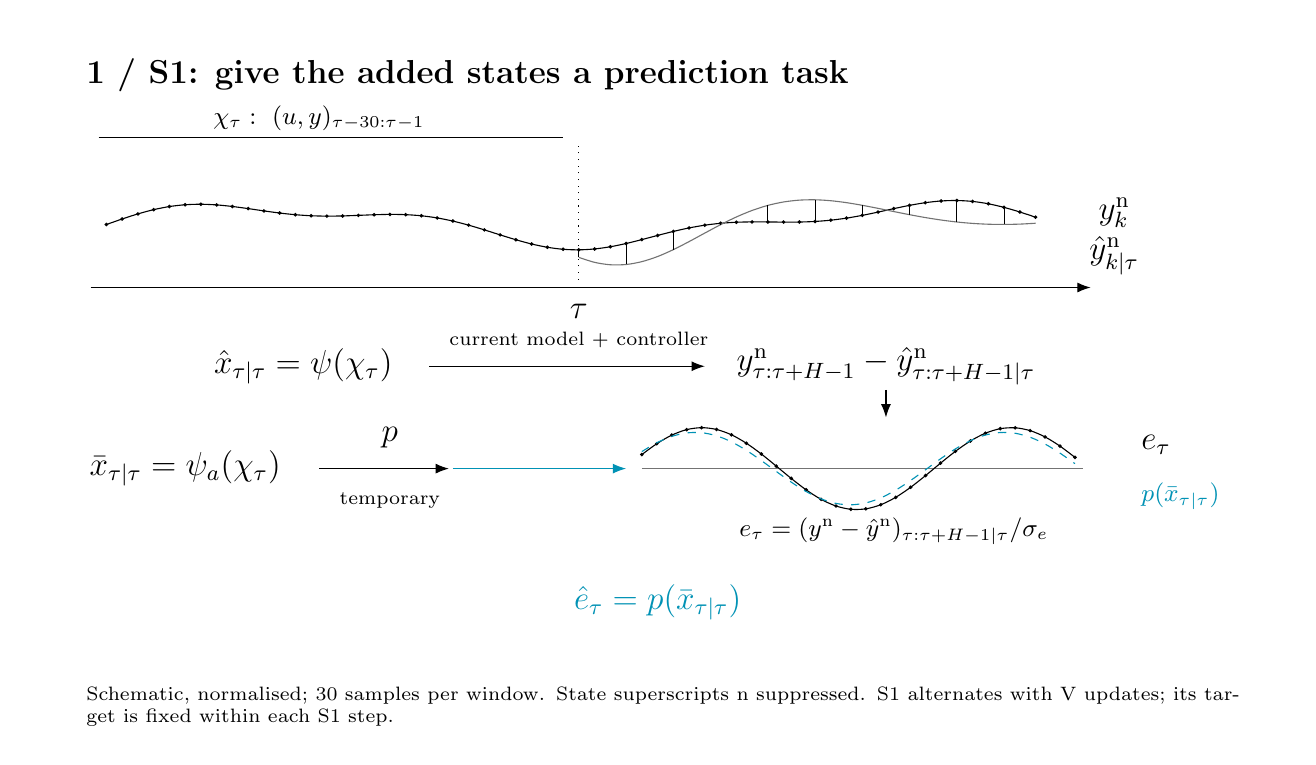
\begin{tikzpicture}\useasboundingbox (0,0) rectangle (16,9);\fill[white] (0,0) rectangle (16,9);\fontsize{12}{14}\selectfont
\node[anchor=west,font=\large\bfseries] at (0.6,8.4) {1 / S1: give the added states a prediction task};
\node[anchor=west,font=\scriptsize,text width=14.8cm,align=left] at (0.6,0.38) {Schematic, normalised; 30 samples per window. State superscripts n suppressed. S1 alternates with V updates; its target is fixed within each S1 step.};
\draw[black] plot[smooth] coordinates {(1.0000,6.5000) (1.2000,6.5703) (1.4000,6.6348) (1.6000,6.6887) (1.8000,6.7281) (2.0000,6.7510) (2.2000,6.7574) (2.4000,6.7490) (2.6000,6.7291) (2.8000,6.7022) (3.0000,6.6730) (3.2000,6.6459) (3.4000,6.6246) (3.6000,6.6113) (3.8000,6.6065) (4.0000,6.6091) (4.2000,6.6162) (4.4000,6.6241) (4.6000,6.6285) (4.8000,6.6252) (5.0000,6.6110) (5.2000,6.5839) (5.4000,6.5437) (5.6000,6.4919) (5.8000,6.4319) (6.0000,6.3684) (6.2000,6.3068) (6.4000,6.2527) (6.6000,6.2110) (6.8000,6.1855) (7.0000,6.1784) (7.2000,6.1897) (7.4000,6.2177) (7.6000,6.2588) (7.8000,6.3085) (8.0000,6.3614) (8.2000,6.4122) (8.4000,6.4567) (8.6000,6.4916) (8.8000,6.5155) (9.0000,6.5287) (9.2000,6.5334) (9.4000,6.5326) (9.6000,6.5306) (9.8000,6.5315) (10.0000,6.5389) (10.2000,6.5551) (10.4000,6.5812) (10.6000,6.6163) (10.8000,6.6577) (11.0000,6.7017) (11.2000,6.7432) (11.4000,6.7772) (11.6000,6.7990) (11.8000,6.8050) (12.0000,6.7932) (12.2000,6.7635) (12.4000,6.7175) (12.6000,6.6591) (12.8000,6.5929)};
\fill[black] (1.0000,6.5000) circle (.025);
\fill[black] (1.2000,6.5703) circle (.025);
\fill[black] (1.4000,6.6348) circle (.025);
\fill[black] (1.6000,6.6887) circle (.025);
\fill[black] (1.8000,6.7281) circle (.025);
\fill[black] (2.0000,6.7510) circle (.025);
\fill[black] (2.2000,6.7574) circle (.025);
\fill[black] (2.4000,6.7490) circle (.025);
\fill[black] (2.6000,6.7291) circle (.025);
\fill[black] (2.8000,6.7022) circle (.025);
\fill[black] (3.0000,6.6730) circle (.025);
\fill[black] (3.2000,6.6459) circle (.025);
\fill[black] (3.4000,6.6246) circle (.025);
\fill[black] (3.6000,6.6113) circle (.025);
\fill[black] (3.8000,6.6065) circle (.025);
\fill[black] (4.0000,6.6091) circle (.025);
\fill[black] (4.2000,6.6162) circle (.025);
\fill[black] (4.4000,6.6241) circle (.025);
\fill[black] (4.6000,6.6285) circle (.025);
\fill[black] (4.8000,6.6252) circle (.025);
\fill[black] (5.0000,6.6110) circle (.025);
\fill[black] (5.2000,6.5839) circle (.025);
\fill[black] (5.4000,6.5437) circle (.025);
\fill[black] (5.6000,6.4919) circle (.025);
\fill[black] (5.8000,6.4319) circle (.025);
\fill[black] (6.0000,6.3684) circle (.025);
\fill[black] (6.2000,6.3068) circle (.025);
\fill[black] (6.4000,6.2527) circle (.025);
\fill[black] (6.6000,6.2110) circle (.025);
\fill[black] (6.8000,6.1855) circle (.025);
\fill[black] (7.0000,6.1784) circle (.025);
\fill[black] (7.2000,6.1897) circle (.025);
\fill[black] (7.4000,6.2177) circle (.025);
\fill[black] (7.6000,6.2588) circle (.025);
\fill[black] (7.8000,6.3085) circle (.025);
\fill[black] (8.0000,6.3614) circle (.025);
\fill[black] (8.2000,6.4122) circle (.025);
\fill[black] (8.4000,6.4567) circle (.025);
\fill[black] (8.6000,6.4916) circle (.025);
\fill[black] (8.8000,6.5155) circle (.025);
\fill[black] (9.0000,6.5287) circle (.025);
\fill[black] (9.2000,6.5334) circle (.025);
\fill[black] (9.4000,6.5326) circle (.025);
\fill[black] (9.6000,6.5306) circle (.025);
\fill[black] (9.8000,6.5315) circle (.025);
\fill[black] (10.0000,6.5389) circle (.025);
\fill[black] (10.2000,6.5551) circle (.025);
\fill[black] (10.4000,6.5812) circle (.025);
\fill[black] (10.6000,6.6163) circle (.025);
\fill[black] (10.8000,6.6577) circle (.025);
\fill[black] (11.0000,6.7017) circle (.025);
\fill[black] (11.2000,6.7432) circle (.025);
\fill[black] (11.4000,6.7772) circle (.025);
\fill[black] (11.6000,6.7990) circle (.025);
\fill[black] (11.8000,6.8050) circle (.025);
\fill[black] (12.0000,6.7932) circle (.025);
\fill[black] (12.2000,6.7635) circle (.025);
\fill[black] (12.4000,6.7175) circle (.025);
\fill[black] (12.6000,6.6591) circle (.025);
\fill[black] (12.8000,6.5929) circle (.025);
\draw[->] (0.8,5.7) -- (13.5,5.7);
\draw[dotted] (7,5.8) -- (7,7.5);
\node[] at (7,5.4) {$\tau$};
\node[] at (13.8,6.65) {$y^{\rm n}_k$};
\draw[] (0.9,7.6) -- (6.8,7.6);
\node[font=\small] at (3.7,7.85) {$\chi_\tau:\ (u,y)_{\tau-30:\tau-1}$};
\draw[black!55] plot[smooth] coordinates {(7.0000,6.0824) (7.2000,6.0195) (7.4000,5.9888) (7.6000,5.9923) (7.8000,6.0285) (8.0000,6.0935) (8.2000,6.1810) (8.4000,6.2832) (8.6000,6.3916) (8.8000,6.4982) (9.0000,6.5957) (9.2000,6.6785) (9.4000,6.7427) (9.6000,6.7864) (9.8000,6.8096) (10.0000,6.8140) (10.2000,6.8021) (10.4000,6.7775) (10.6000,6.7439) (10.8000,6.7051) (11.0000,6.6645) (11.2000,6.6248) (11.4000,6.5884) (11.6000,6.5571) (11.8000,6.5320) (12.0000,6.5141) (12.2000,6.5037) (12.4000,6.5009) (12.6000,6.5052) (12.8000,6.5160)};
\node[black] at (13.8,6.1) {$\hat y^{\rm n}_{k|\tau}$};
\node[black] at (3.5,4.7) {$\hat x_{\tau|\tau}=\psi(\chi_\tau)$};
\draw[black,->] (5.1,4.7) -- (8.6,4.7);
\node[font=\scriptsize,black] at (7,5.03) {current model + controller};
\node[black] at (10.9,4.7) {$y^{\rm n}_{\tau:\tau+H-1}-\hat y^{\rm n}_{\tau:\tau+H-1|\tau}$};
\draw[black] (7.0,6.1784) -- (7.0,6.0824);
\draw[black] (7.6,6.2588) -- (7.6,5.9923);
\draw[black] (8.2,6.4122) -- (8.2,6.181);
\draw[black] (8.8,6.5155) -- (8.8,6.4982);
\draw[black] (9.4,6.5326) -- (9.4,6.7427);
\draw[black] (10.0,6.5389) -- (10.0,6.814);
\draw[black] (10.6,6.6163) -- (10.6,6.7439);
\draw[black] (11.2,6.7432) -- (11.2,6.6248);
\draw[black] (11.8,6.805) -- (11.8,6.532);
\draw[black] (12.4,6.7175) -- (12.4,6.5009);
\draw[black!55] (7.8,3.4) -- (13.4,3.4);
\draw[black] plot[smooth] coordinates {(7.8000,3.5783) (7.9897,3.7161) (8.1793,3.8250) (8.3690,3.8951) (8.5586,3.9200) (8.7483,3.8974) (8.9379,3.8294) (9.1276,3.7222) (9.3172,3.5856) (9.5069,3.4320) (9.6966,3.2756) (9.8862,3.1304) (10.0759,3.0099) (10.2655,2.9250) (10.4552,2.8835) (10.6448,2.8891) (10.8345,2.9414) (11.0241,3.0355) (11.2138,3.1630) (11.4034,3.3120) (11.5931,3.4691) (11.7828,3.6199) (11.9724,3.7506) (12.1621,3.8493) (12.3517,3.9070) (12.5414,3.9184) (12.7310,3.8824) (12.9207,3.8024) (13.1103,3.6857) (13.3000,3.5429)};
\fill[black] (7.8000,3.5783) circle (.025);
\fill[black] (7.9897,3.7161) circle (.025);
\fill[black] (8.1793,3.8250) circle (.025);
\fill[black] (8.3690,3.8951) circle (.025);
\fill[black] (8.5586,3.9200) circle (.025);
\fill[black] (8.7483,3.8974) circle (.025);
\fill[black] (8.9379,3.8294) circle (.025);
\fill[black] (9.1276,3.7222) circle (.025);
\fill[black] (9.3172,3.5856) circle (.025);
\fill[black] (9.5069,3.4320) circle (.025);
\fill[black] (9.6966,3.2756) circle (.025);
\fill[black] (9.8862,3.1304) circle (.025);
\fill[black] (10.0759,3.0099) circle (.025);
\fill[black] (10.2655,2.9250) circle (.025);
\fill[black] (10.4552,2.8835) circle (.025);
\fill[black] (10.6448,2.8891) circle (.025);
\fill[black] (10.8345,2.9414) circle (.025);
\fill[black] (11.0241,3.0355) circle (.025);
\fill[black] (11.2138,3.1630) circle (.025);
\fill[black] (11.4034,3.3120) circle (.025);
\fill[black] (11.5931,3.4691) circle (.025);
\fill[black] (11.7828,3.6199) circle (.025);
\fill[black] (11.9724,3.7506) circle (.025);
\fill[black] (12.1621,3.8493) circle (.025);
\fill[black] (12.3517,3.9070) circle (.025);
\fill[black] (12.5414,3.9184) circle (.025);
\fill[black] (12.7310,3.8824) circle (.025);
\fill[black] (12.9207,3.8024) circle (.025);
\fill[black] (13.1103,3.6857) circle (.025);
\fill[black] (13.3000,3.5429) circle (.025);
\node[anchor=west,black] at (14,3.7) {$e_\tau$};
\draw[->,black] (10.9,4.4) -- (10.9,4.05);
\node[black,font=\small] at (11,2.6) {$e_\tau=(y^{\rm n}-\hat y^{\rm n})_{\tau:\tau+H-1|\tau}/\sigma_e$};
\node[black] at (2,3.4) {$\bar x_{\tau|\tau}=\psi_a(\chi_\tau)$};
\draw[->,black] (3.7,3.4) -- (5.35,3.4);
\node[font=\large,black] at (4.6,3.8) {$p$};
\node[font=\scriptsize,black] at (4.6,3) {temporary};
\draw[hl,dashed] plot[smooth] coordinates {(7.8000,3.6165) (7.9897,3.7278) (8.1793,3.8093) (8.3690,3.8533) (8.5586,3.8560) (8.7483,3.8170) (8.9379,3.7400) (9.1276,3.6319) (9.3172,3.5026) (9.5069,3.3640) (9.6966,3.2287) (9.8862,3.1090) (10.0759,3.0159) (10.2655,2.9578) (10.4552,2.9401) (10.6448,2.9644) (10.8345,3.0285) (11.0241,3.1265) (11.2138,3.2495) (11.4034,3.3862) (11.5931,3.5242) (11.7828,3.6508) (11.9724,3.7545) (12.1621,3.8259) (12.3517,3.8584) (12.5414,3.8490) (12.7310,3.7986) (12.9207,3.7119) (13.1103,3.5966) (13.3000,3.4634)};
\draw[->,hl] (5.4,3.4) -- (7.6,3.4);
\node[anchor=west,hl,font=\small] at (14,3.05) {$p(\bar x_{\tau|\tau})$};
\node[hl] at (8,1.7) {$\hat e_\tau=p(\bar x_{\tau|\tau})$};
\end{tikzpicture}
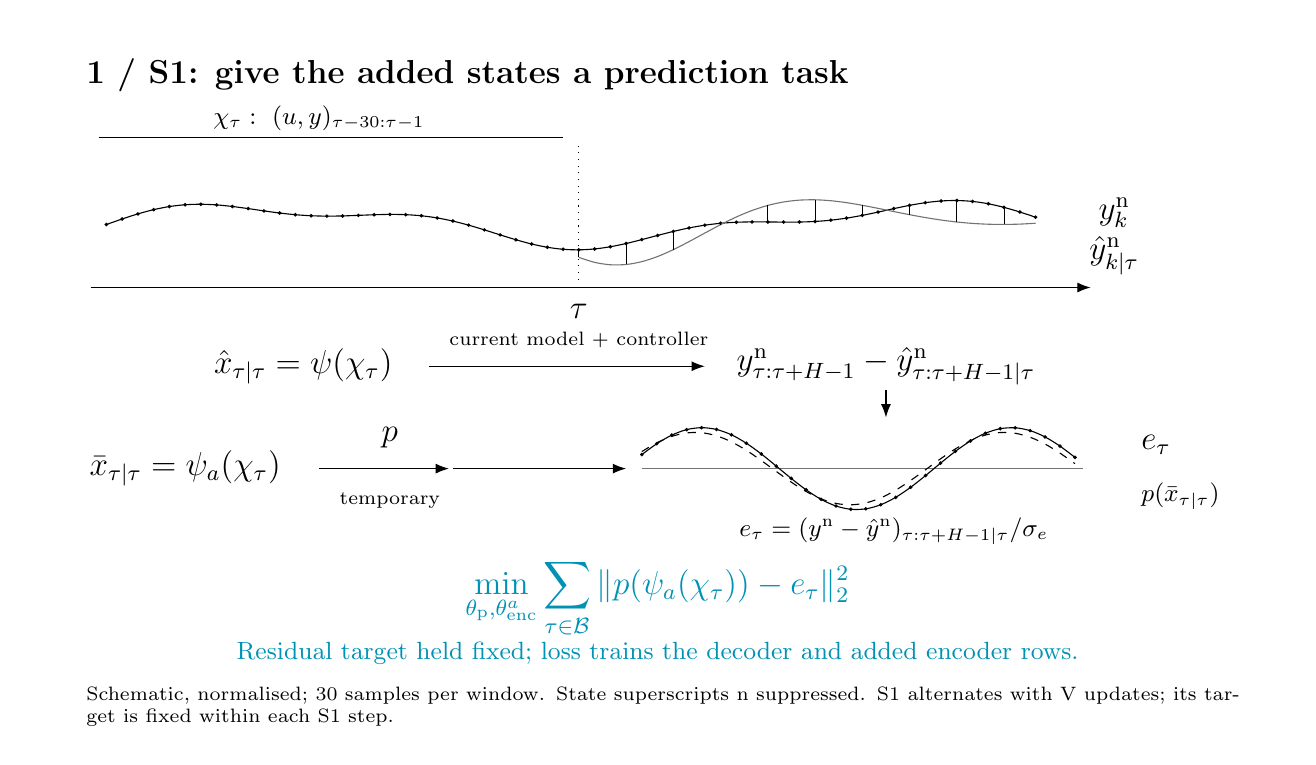
\begin{tikzpicture}\useasboundingbox (0,0) rectangle (16,9);\fill[white] (0,0) rectangle (16,9);\fontsize{12}{14}\selectfont
\node[anchor=west,font=\large\bfseries] at (0.6,8.4) {1 / S1: give the added states a prediction task};
\node[anchor=west,font=\scriptsize,text width=14.8cm,align=left] at (0.6,0.38) {Schematic, normalised; 30 samples per window. State superscripts n suppressed. S1 alternates with V updates; its target is fixed within each S1 step.};
\draw[black] plot[smooth] coordinates {(1.0000,6.5000) (1.2000,6.5703) (1.4000,6.6348) (1.6000,6.6887) (1.8000,6.7281) (2.0000,6.7510) (2.2000,6.7574) (2.4000,6.7490) (2.6000,6.7291) (2.8000,6.7022) (3.0000,6.6730) (3.2000,6.6459) (3.4000,6.6246) (3.6000,6.6113) (3.8000,6.6065) (4.0000,6.6091) (4.2000,6.6162) (4.4000,6.6241) (4.6000,6.6285) (4.8000,6.6252) (5.0000,6.6110) (5.2000,6.5839) (5.4000,6.5437) (5.6000,6.4919) (5.8000,6.4319) (6.0000,6.3684) (6.2000,6.3068) (6.4000,6.2527) (6.6000,6.2110) (6.8000,6.1855) (7.0000,6.1784) (7.2000,6.1897) (7.4000,6.2177) (7.6000,6.2588) (7.8000,6.3085) (8.0000,6.3614) (8.2000,6.4122) (8.4000,6.4567) (8.6000,6.4916) (8.8000,6.5155) (9.0000,6.5287) (9.2000,6.5334) (9.4000,6.5326) (9.6000,6.5306) (9.8000,6.5315) (10.0000,6.5389) (10.2000,6.5551) (10.4000,6.5812) (10.6000,6.6163) (10.8000,6.6577) (11.0000,6.7017) (11.2000,6.7432) (11.4000,6.7772) (11.6000,6.7990) (11.8000,6.8050) (12.0000,6.7932) (12.2000,6.7635) (12.4000,6.7175) (12.6000,6.6591) (12.8000,6.5929)};
\fill[black] (1.0000,6.5000) circle (.025);
\fill[black] (1.2000,6.5703) circle (.025);
\fill[black] (1.4000,6.6348) circle (.025);
\fill[black] (1.6000,6.6887) circle (.025);
\fill[black] (1.8000,6.7281) circle (.025);
\fill[black] (2.0000,6.7510) circle (.025);
\fill[black] (2.2000,6.7574) circle (.025);
\fill[black] (2.4000,6.7490) circle (.025);
\fill[black] (2.6000,6.7291) circle (.025);
\fill[black] (2.8000,6.7022) circle (.025);
\fill[black] (3.0000,6.6730) circle (.025);
\fill[black] (3.2000,6.6459) circle (.025);
\fill[black] (3.4000,6.6246) circle (.025);
\fill[black] (3.6000,6.6113) circle (.025);
\fill[black] (3.8000,6.6065) circle (.025);
\fill[black] (4.0000,6.6091) circle (.025);
\fill[black] (4.2000,6.6162) circle (.025);
\fill[black] (4.4000,6.6241) circle (.025);
\fill[black] (4.6000,6.6285) circle (.025);
\fill[black] (4.8000,6.6252) circle (.025);
\fill[black] (5.0000,6.6110) circle (.025);
\fill[black] (5.2000,6.5839) circle (.025);
\fill[black] (5.4000,6.5437) circle (.025);
\fill[black] (5.6000,6.4919) circle (.025);
\fill[black] (5.8000,6.4319) circle (.025);
\fill[black] (6.0000,6.3684) circle (.025);
\fill[black] (6.2000,6.3068) circle (.025);
\fill[black] (6.4000,6.2527) circle (.025);
\fill[black] (6.6000,6.2110) circle (.025);
\fill[black] (6.8000,6.1855) circle (.025);
\fill[black] (7.0000,6.1784) circle (.025);
\fill[black] (7.2000,6.1897) circle (.025);
\fill[black] (7.4000,6.2177) circle (.025);
\fill[black] (7.6000,6.2588) circle (.025);
\fill[black] (7.8000,6.3085) circle (.025);
\fill[black] (8.0000,6.3614) circle (.025);
\fill[black] (8.2000,6.4122) circle (.025);
\fill[black] (8.4000,6.4567) circle (.025);
\fill[black] (8.6000,6.4916) circle (.025);
\fill[black] (8.8000,6.5155) circle (.025);
\fill[black] (9.0000,6.5287) circle (.025);
\fill[black] (9.2000,6.5334) circle (.025);
\fill[black] (9.4000,6.5326) circle (.025);
\fill[black] (9.6000,6.5306) circle (.025);
\fill[black] (9.8000,6.5315) circle (.025);
\fill[black] (10.0000,6.5389) circle (.025);
\fill[black] (10.2000,6.5551) circle (.025);
\fill[black] (10.4000,6.5812) circle (.025);
\fill[black] (10.6000,6.6163) circle (.025);
\fill[black] (10.8000,6.6577) circle (.025);
\fill[black] (11.0000,6.7017) circle (.025);
\fill[black] (11.2000,6.7432) circle (.025);
\fill[black] (11.4000,6.7772) circle (.025);
\fill[black] (11.6000,6.7990) circle (.025);
\fill[black] (11.8000,6.8050) circle (.025);
\fill[black] (12.0000,6.7932) circle (.025);
\fill[black] (12.2000,6.7635) circle (.025);
\fill[black] (12.4000,6.7175) circle (.025);
\fill[black] (12.6000,6.6591) circle (.025);
\fill[black] (12.8000,6.5929) circle (.025);
\draw[->] (0.8,5.7) -- (13.5,5.7);
\draw[dotted] (7,5.8) -- (7,7.5);
\node[] at (7,5.4) {$\tau$};
\node[] at (13.8,6.65) {$y^{\rm n}_k$};
\draw[] (0.9,7.6) -- (6.8,7.6);
\node[font=\small] at (3.7,7.85) {$\chi_\tau:\ (u,y)_{\tau-30:\tau-1}$};
\draw[black!55] plot[smooth] coordinates {(7.0000,6.0824) (7.2000,6.0195) (7.4000,5.9888) (7.6000,5.9923) (7.8000,6.0285) (8.0000,6.0935) (8.2000,6.1810) (8.4000,6.2832) (8.6000,6.3916) (8.8000,6.4982) (9.0000,6.5957) (9.2000,6.6785) (9.4000,6.7427) (9.6000,6.7864) (9.8000,6.8096) (10.0000,6.8140) (10.2000,6.8021) (10.4000,6.7775) (10.6000,6.7439) (10.8000,6.7051) (11.0000,6.6645) (11.2000,6.6248) (11.4000,6.5884) (11.6000,6.5571) (11.8000,6.5320) (12.0000,6.5141) (12.2000,6.5037) (12.4000,6.5009) (12.6000,6.5052) (12.8000,6.5160)};
\node[black] at (13.8,6.1) {$\hat y^{\rm n}_{k|\tau}$};
\node[black] at (3.5,4.7) {$\hat x_{\tau|\tau}=\psi(\chi_\tau)$};
\draw[black,->] (5.1,4.7) -- (8.6,4.7);
\node[font=\scriptsize,black] at (7,5.03) {current model + controller};
\node[black] at (10.9,4.7) {$y^{\rm n}_{\tau:\tau+H-1}-\hat y^{\rm n}_{\tau:\tau+H-1|\tau}$};
\draw[black] (7.0,6.1784) -- (7.0,6.0824);
\draw[black] (7.6,6.2588) -- (7.6,5.9923);
\draw[black] (8.2,6.4122) -- (8.2,6.181);
\draw[black] (8.8,6.5155) -- (8.8,6.4982);
\draw[black] (9.4,6.5326) -- (9.4,6.7427);
\draw[black] (10.0,6.5389) -- (10.0,6.814);
\draw[black] (10.6,6.6163) -- (10.6,6.7439);
\draw[black] (11.2,6.7432) -- (11.2,6.6248);
\draw[black] (11.8,6.805) -- (11.8,6.532);
\draw[black] (12.4,6.7175) -- (12.4,6.5009);
\draw[black!55] (7.8,3.4) -- (13.4,3.4);
\draw[black] plot[smooth] coordinates {(7.8000,3.5783) (7.9897,3.7161) (8.1793,3.8250) (8.3690,3.8951) (8.5586,3.9200) (8.7483,3.8974) (8.9379,3.8294) (9.1276,3.7222) (9.3172,3.5856) (9.5069,3.4320) (9.6966,3.2756) (9.8862,3.1304) (10.0759,3.0099) (10.2655,2.9250) (10.4552,2.8835) (10.6448,2.8891) (10.8345,2.9414) (11.0241,3.0355) (11.2138,3.1630) (11.4034,3.3120) (11.5931,3.4691) (11.7828,3.6199) (11.9724,3.7506) (12.1621,3.8493) (12.3517,3.9070) (12.5414,3.9184) (12.7310,3.8824) (12.9207,3.8024) (13.1103,3.6857) (13.3000,3.5429)};
\fill[black] (7.8000,3.5783) circle (.025);
\fill[black] (7.9897,3.7161) circle (.025);
\fill[black] (8.1793,3.8250) circle (.025);
\fill[black] (8.3690,3.8951) circle (.025);
\fill[black] (8.5586,3.9200) circle (.025);
\fill[black] (8.7483,3.8974) circle (.025);
\fill[black] (8.9379,3.8294) circle (.025);
\fill[black] (9.1276,3.7222) circle (.025);
\fill[black] (9.3172,3.5856) circle (.025);
\fill[black] (9.5069,3.4320) circle (.025);
\fill[black] (9.6966,3.2756) circle (.025);
\fill[black] (9.8862,3.1304) circle (.025);
\fill[black] (10.0759,3.0099) circle (.025);
\fill[black] (10.2655,2.9250) circle (.025);
\fill[black] (10.4552,2.8835) circle (.025);
\fill[black] (10.6448,2.8891) circle (.025);
\fill[black] (10.8345,2.9414) circle (.025);
\fill[black] (11.0241,3.0355) circle (.025);
\fill[black] (11.2138,3.1630) circle (.025);
\fill[black] (11.4034,3.3120) circle (.025);
\fill[black] (11.5931,3.4691) circle (.025);
\fill[black] (11.7828,3.6199) circle (.025);
\fill[black] (11.9724,3.7506) circle (.025);
\fill[black] (12.1621,3.8493) circle (.025);
\fill[black] (12.3517,3.9070) circle (.025);
\fill[black] (12.5414,3.9184) circle (.025);
\fill[black] (12.7310,3.8824) circle (.025);
\fill[black] (12.9207,3.8024) circle (.025);
\fill[black] (13.1103,3.6857) circle (.025);
\fill[black] (13.3000,3.5429) circle (.025);
\node[anchor=west,black] at (14,3.7) {$e_\tau$};
\draw[->,black] (10.9,4.4) -- (10.9,4.05);
\node[black,font=\small] at (11,2.6) {$e_\tau=(y^{\rm n}-\hat y^{\rm n})_{\tau:\tau+H-1|\tau}/\sigma_e$};
\node[black] at (2,3.4) {$\bar x_{\tau|\tau}=\psi_a(\chi_\tau)$};
\draw[->,black] (3.7,3.4) -- (5.35,3.4);
\node[font=\large,black] at (4.6,3.8) {$p$};
\node[font=\scriptsize,black] at (4.6,3) {temporary};
\draw[black,dashed] plot[smooth] coordinates {(7.8000,3.6165) (7.9897,3.7278) (8.1793,3.8093) (8.3690,3.8533) (8.5586,3.8560) (8.7483,3.8170) (8.9379,3.7400) (9.1276,3.6319) (9.3172,3.5026) (9.5069,3.3640) (9.6966,3.2287) (9.8862,3.1090) (10.0759,3.0159) (10.2655,2.9578) (10.4552,2.9401) (10.6448,2.9644) (10.8345,3.0285) (11.0241,3.1265) (11.2138,3.2495) (11.4034,3.3862) (11.5931,3.5242) (11.7828,3.6508) (11.9724,3.7545) (12.1621,3.8259) (12.3517,3.8584) (12.5414,3.8490) (12.7310,3.7986) (12.9207,3.7119) (13.1103,3.5966) (13.3000,3.4634)};
\draw[->,black] (5.4,3.4) -- (7.6,3.4);
\node[anchor=west,black,font=\small] at (14,3.05) {$p(\bar x_{\tau|\tau})$};
\node[hl] at (8,1.75) {$\displaystyle\min_{\theta_{\rm p},\theta^a_{\rm enc}}\sum_{\tau\in\mathcal B}\|p(\psi_a(\chi_\tau))-e_\tau\|_2^2$};
\node[font=\small,hl] at (8,1.05) {Residual target held fixed; loss trains the decoder and added encoder rows.};
\end{tikzpicture}
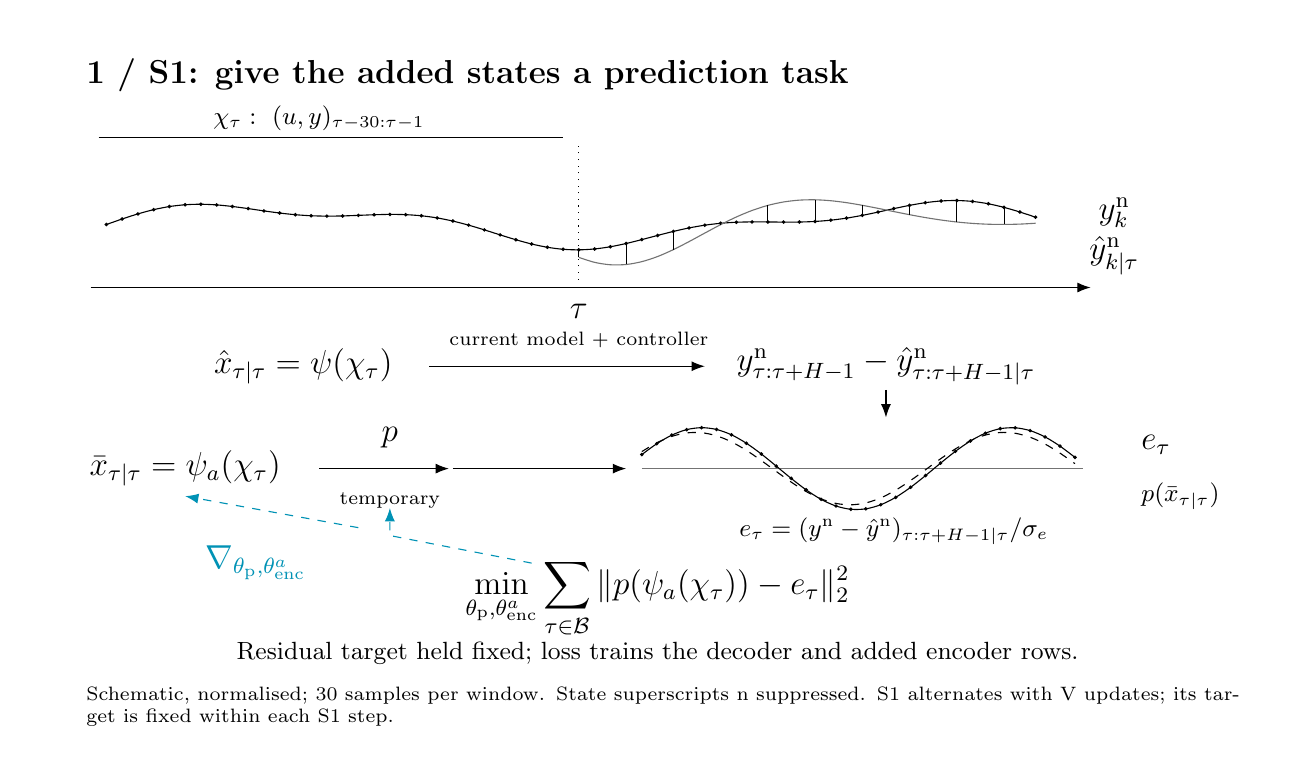
\begin{tikzpicture}\useasboundingbox (0,0) rectangle (16,9);\fill[white] (0,0) rectangle (16,9);\fontsize{12}{14}\selectfont
\node[anchor=west,font=\large\bfseries] at (0.6,8.4) {1 / S1: give the added states a prediction task};
\node[anchor=west,font=\scriptsize,text width=14.8cm,align=left] at (0.6,0.38) {Schematic, normalised; 30 samples per window. State superscripts n suppressed. S1 alternates with V updates; its target is fixed within each S1 step.};
\draw[black] plot[smooth] coordinates {(1.0000,6.5000) (1.2000,6.5703) (1.4000,6.6348) (1.6000,6.6887) (1.8000,6.7281) (2.0000,6.7510) (2.2000,6.7574) (2.4000,6.7490) (2.6000,6.7291) (2.8000,6.7022) (3.0000,6.6730) (3.2000,6.6459) (3.4000,6.6246) (3.6000,6.6113) (3.8000,6.6065) (4.0000,6.6091) (4.2000,6.6162) (4.4000,6.6241) (4.6000,6.6285) (4.8000,6.6252) (5.0000,6.6110) (5.2000,6.5839) (5.4000,6.5437) (5.6000,6.4919) (5.8000,6.4319) (6.0000,6.3684) (6.2000,6.3068) (6.4000,6.2527) (6.6000,6.2110) (6.8000,6.1855) (7.0000,6.1784) (7.2000,6.1897) (7.4000,6.2177) (7.6000,6.2588) (7.8000,6.3085) (8.0000,6.3614) (8.2000,6.4122) (8.4000,6.4567) (8.6000,6.4916) (8.8000,6.5155) (9.0000,6.5287) (9.2000,6.5334) (9.4000,6.5326) (9.6000,6.5306) (9.8000,6.5315) (10.0000,6.5389) (10.2000,6.5551) (10.4000,6.5812) (10.6000,6.6163) (10.8000,6.6577) (11.0000,6.7017) (11.2000,6.7432) (11.4000,6.7772) (11.6000,6.7990) (11.8000,6.8050) (12.0000,6.7932) (12.2000,6.7635) (12.4000,6.7175) (12.6000,6.6591) (12.8000,6.5929)};
\fill[black] (1.0000,6.5000) circle (.025);
\fill[black] (1.2000,6.5703) circle (.025);
\fill[black] (1.4000,6.6348) circle (.025);
\fill[black] (1.6000,6.6887) circle (.025);
\fill[black] (1.8000,6.7281) circle (.025);
\fill[black] (2.0000,6.7510) circle (.025);
\fill[black] (2.2000,6.7574) circle (.025);
\fill[black] (2.4000,6.7490) circle (.025);
\fill[black] (2.6000,6.7291) circle (.025);
\fill[black] (2.8000,6.7022) circle (.025);
\fill[black] (3.0000,6.6730) circle (.025);
\fill[black] (3.2000,6.6459) circle (.025);
\fill[black] (3.4000,6.6246) circle (.025);
\fill[black] (3.6000,6.6113) circle (.025);
\fill[black] (3.8000,6.6065) circle (.025);
\fill[black] (4.0000,6.6091) circle (.025);
\fill[black] (4.2000,6.6162) circle (.025);
\fill[black] (4.4000,6.6241) circle (.025);
\fill[black] (4.6000,6.6285) circle (.025);
\fill[black] (4.8000,6.6252) circle (.025);
\fill[black] (5.0000,6.6110) circle (.025);
\fill[black] (5.2000,6.5839) circle (.025);
\fill[black] (5.4000,6.5437) circle (.025);
\fill[black] (5.6000,6.4919) circle (.025);
\fill[black] (5.8000,6.4319) circle (.025);
\fill[black] (6.0000,6.3684) circle (.025);
\fill[black] (6.2000,6.3068) circle (.025);
\fill[black] (6.4000,6.2527) circle (.025);
\fill[black] (6.6000,6.2110) circle (.025);
\fill[black] (6.8000,6.1855) circle (.025);
\fill[black] (7.0000,6.1784) circle (.025);
\fill[black] (7.2000,6.1897) circle (.025);
\fill[black] (7.4000,6.2177) circle (.025);
\fill[black] (7.6000,6.2588) circle (.025);
\fill[black] (7.8000,6.3085) circle (.025);
\fill[black] (8.0000,6.3614) circle (.025);
\fill[black] (8.2000,6.4122) circle (.025);
\fill[black] (8.4000,6.4567) circle (.025);
\fill[black] (8.6000,6.4916) circle (.025);
\fill[black] (8.8000,6.5155) circle (.025);
\fill[black] (9.0000,6.5287) circle (.025);
\fill[black] (9.2000,6.5334) circle (.025);
\fill[black] (9.4000,6.5326) circle (.025);
\fill[black] (9.6000,6.5306) circle (.025);
\fill[black] (9.8000,6.5315) circle (.025);
\fill[black] (10.0000,6.5389) circle (.025);
\fill[black] (10.2000,6.5551) circle (.025);
\fill[black] (10.4000,6.5812) circle (.025);
\fill[black] (10.6000,6.6163) circle (.025);
\fill[black] (10.8000,6.6577) circle (.025);
\fill[black] (11.0000,6.7017) circle (.025);
\fill[black] (11.2000,6.7432) circle (.025);
\fill[black] (11.4000,6.7772) circle (.025);
\fill[black] (11.6000,6.7990) circle (.025);
\fill[black] (11.8000,6.8050) circle (.025);
\fill[black] (12.0000,6.7932) circle (.025);
\fill[black] (12.2000,6.7635) circle (.025);
\fill[black] (12.4000,6.7175) circle (.025);
\fill[black] (12.6000,6.6591) circle (.025);
\fill[black] (12.8000,6.5929) circle (.025);
\draw[->] (0.8,5.7) -- (13.5,5.7);
\draw[dotted] (7,5.8) -- (7,7.5);
\node[] at (7,5.4) {$\tau$};
\node[] at (13.8,6.65) {$y^{\rm n}_k$};
\draw[] (0.9,7.6) -- (6.8,7.6);
\node[font=\small] at (3.7,7.85) {$\chi_\tau:\ (u,y)_{\tau-30:\tau-1}$};
\draw[black!55] plot[smooth] coordinates {(7.0000,6.0824) (7.2000,6.0195) (7.4000,5.9888) (7.6000,5.9923) (7.8000,6.0285) (8.0000,6.0935) (8.2000,6.1810) (8.4000,6.2832) (8.6000,6.3916) (8.8000,6.4982) (9.0000,6.5957) (9.2000,6.6785) (9.4000,6.7427) (9.6000,6.7864) (9.8000,6.8096) (10.0000,6.8140) (10.2000,6.8021) (10.4000,6.7775) (10.6000,6.7439) (10.8000,6.7051) (11.0000,6.6645) (11.2000,6.6248) (11.4000,6.5884) (11.6000,6.5571) (11.8000,6.5320) (12.0000,6.5141) (12.2000,6.5037) (12.4000,6.5009) (12.6000,6.5052) (12.8000,6.5160)};
\node[black] at (13.8,6.1) {$\hat y^{\rm n}_{k|\tau}$};
\node[black] at (3.5,4.7) {$\hat x_{\tau|\tau}=\psi(\chi_\tau)$};
\draw[black,->] (5.1,4.7) -- (8.6,4.7);
\node[font=\scriptsize,black] at (7,5.03) {current model + controller};
\node[black] at (10.9,4.7) {$y^{\rm n}_{\tau:\tau+H-1}-\hat y^{\rm n}_{\tau:\tau+H-1|\tau}$};
\draw[black] (7.0,6.1784) -- (7.0,6.0824);
\draw[black] (7.6,6.2588) -- (7.6,5.9923);
\draw[black] (8.2,6.4122) -- (8.2,6.181);
\draw[black] (8.8,6.5155) -- (8.8,6.4982);
\draw[black] (9.4,6.5326) -- (9.4,6.7427);
\draw[black] (10.0,6.5389) -- (10.0,6.814);
\draw[black] (10.6,6.6163) -- (10.6,6.7439);
\draw[black] (11.2,6.7432) -- (11.2,6.6248);
\draw[black] (11.8,6.805) -- (11.8,6.532);
\draw[black] (12.4,6.7175) -- (12.4,6.5009);
\draw[black!55] (7.8,3.4) -- (13.4,3.4);
\draw[black] plot[smooth] coordinates {(7.8000,3.5783) (7.9897,3.7161) (8.1793,3.8250) (8.3690,3.8951) (8.5586,3.9200) (8.7483,3.8974) (8.9379,3.8294) (9.1276,3.7222) (9.3172,3.5856) (9.5069,3.4320) (9.6966,3.2756) (9.8862,3.1304) (10.0759,3.0099) (10.2655,2.9250) (10.4552,2.8835) (10.6448,2.8891) (10.8345,2.9414) (11.0241,3.0355) (11.2138,3.1630) (11.4034,3.3120) (11.5931,3.4691) (11.7828,3.6199) (11.9724,3.7506) (12.1621,3.8493) (12.3517,3.9070) (12.5414,3.9184) (12.7310,3.8824) (12.9207,3.8024) (13.1103,3.6857) (13.3000,3.5429)};
\fill[black] (7.8000,3.5783) circle (.025);
\fill[black] (7.9897,3.7161) circle (.025);
\fill[black] (8.1793,3.8250) circle (.025);
\fill[black] (8.3690,3.8951) circle (.025);
\fill[black] (8.5586,3.9200) circle (.025);
\fill[black] (8.7483,3.8974) circle (.025);
\fill[black] (8.9379,3.8294) circle (.025);
\fill[black] (9.1276,3.7222) circle (.025);
\fill[black] (9.3172,3.5856) circle (.025);
\fill[black] (9.5069,3.4320) circle (.025);
\fill[black] (9.6966,3.2756) circle (.025);
\fill[black] (9.8862,3.1304) circle (.025);
\fill[black] (10.0759,3.0099) circle (.025);
\fill[black] (10.2655,2.9250) circle (.025);
\fill[black] (10.4552,2.8835) circle (.025);
\fill[black] (10.6448,2.8891) circle (.025);
\fill[black] (10.8345,2.9414) circle (.025);
\fill[black] (11.0241,3.0355) circle (.025);
\fill[black] (11.2138,3.1630) circle (.025);
\fill[black] (11.4034,3.3120) circle (.025);
\fill[black] (11.5931,3.4691) circle (.025);
\fill[black] (11.7828,3.6199) circle (.025);
\fill[black] (11.9724,3.7506) circle (.025);
\fill[black] (12.1621,3.8493) circle (.025);
\fill[black] (12.3517,3.9070) circle (.025);
\fill[black] (12.5414,3.9184) circle (.025);
\fill[black] (12.7310,3.8824) circle (.025);
\fill[black] (12.9207,3.8024) circle (.025);
\fill[black] (13.1103,3.6857) circle (.025);
\fill[black] (13.3000,3.5429) circle (.025);
\node[anchor=west,black] at (14,3.7) {$e_\tau$};
\draw[->,black] (10.9,4.4) -- (10.9,4.05);
\node[black,font=\small] at (11,2.6) {$e_\tau=(y^{\rm n}-\hat y^{\rm n})_{\tau:\tau+H-1|\tau}/\sigma_e$};
\node[black] at (2,3.4) {$\bar x_{\tau|\tau}=\psi_a(\chi_\tau)$};
\draw[->,black] (3.7,3.4) -- (5.35,3.4);
\node[font=\large,black] at (4.6,3.8) {$p$};
\node[font=\scriptsize,black] at (4.6,3) {temporary};
\draw[black,dashed] plot[smooth] coordinates {(7.8000,3.6165) (7.9897,3.7278) (8.1793,3.8093) (8.3690,3.8533) (8.5586,3.8560) (8.7483,3.8170) (8.9379,3.7400) (9.1276,3.6319) (9.3172,3.5026) (9.5069,3.3640) (9.6966,3.2287) (9.8862,3.1090) (10.0759,3.0159) (10.2655,2.9578) (10.4552,2.9401) (10.6448,2.9644) (10.8345,3.0285) (11.0241,3.1265) (11.2138,3.2495) (11.4034,3.3862) (11.5931,3.5242) (11.7828,3.6508) (11.9724,3.7545) (12.1621,3.8259) (12.3517,3.8584) (12.5414,3.8490) (12.7310,3.7986) (12.9207,3.7119) (13.1103,3.5966) (13.3000,3.4634)};
\draw[->,black] (5.4,3.4) -- (7.6,3.4);
\node[anchor=west,black,font=\small] at (14,3.05) {$p(\bar x_{\tau|\tau})$};
\node[black] at (8,1.75) {$\displaystyle\min_{\theta_{\rm p},\theta^a_{\rm enc}}\sum_{\tau\in\mathcal B}\|p(\psi_a(\chi_\tau))-e_\tau\|_2^2$};
\node[font=\small,black] at (8,1.05) {Residual target held fixed; loss trains the decoder and added encoder rows.};
\draw[->,hl,dashed] (6.4,2.2) -- (4.6,2.55) -- (4.6,2.9);\draw[->,hl,dashed] (4.2,2.65) -- (2,3.05);
\node[hl] at (2.9,2.2) {$\nabla_{\theta_{\rm p},\theta^a_{\rm enc}}$};
\end{tikzpicture}
\begin{tikzpicture}\useasboundingbox (0,0) rectangle (16,9);\fill[white] (0,0) rectangle (16,9);\fontsize{12}{14}\selectfont
\node[anchor=west,font=\large\bfseries] at (0.6,8.4) {1 / S2: predict the next encoded state};
\node[anchor=west,font=\scriptsize,text width=14.8cm,align=left] at (0.6,0.38) {Schematic; only the last few data samples shown. Grey encoder routes and targets are fixed throughout S2.};
\fill (1.0,6.700) circle (.045);
\fill (1.65,6.910) circle (.045);
\fill (2.3,6.927) circle (.045);
\fill (2.95,6.735) circle (.045);
\fill (3.6,6.511) circle (.045);
\fill (4.25,6.460) circle (.045);
\fill (4.9,6.630) circle (.045);
\fill (5.55,6.864) circle (.045);
\fill (6.2,6.947) circle (.045);
\node[] at (5.45,7.15) {$\tau-1$};
\node[] at (6.35,7.15) {$\tau$};
\draw[hl] (1,6.1) -- (5.55,6.1);
\node[] at (3,5.8) {$\chi_\tau$};
\node[hl] at (8,1.75) {$\chi_\tau=(u,y)_{\tau-30:\tau-1}$};
\end{tikzpicture}
\begin{tikzpicture}\useasboundingbox (0,0) rectangle (16,9);\fill[white] (0,0) rectangle (16,9);\fontsize{12}{14}\selectfont
\node[anchor=west,font=\large\bfseries] at (0.6,8.4) {1 / S2: predict the next encoded state};
\node[anchor=west,font=\scriptsize,text width=14.8cm,align=left] at (0.6,0.38) {Schematic; only the last few data samples shown. Grey encoder routes and targets are fixed throughout S2.};
\fill (1.0,6.700) circle (.045);
\fill (1.65,6.910) circle (.045);
\fill (2.3,6.927) circle (.045);
\fill (2.95,6.735) circle (.045);
\fill (3.6,6.511) circle (.045);
\fill (4.25,6.460) circle (.045);
\fill (4.9,6.630) circle (.045);
\fill (5.55,6.864) circle (.045);
\fill (6.2,6.947) circle (.045);
\node[] at (5.45,7.15) {$\tau-1$};
\node[] at (6.35,7.15) {$\tau$};
\draw[black] (1,6.1) -- (5.55,6.1);
\node[] at (3,5.8) {$\chi_\tau$};
\draw[hl] (1.65,5.3) -- (6.2,5.3);
\node[hl] at (3.5,5) {$\chi_{\tau+1}$};
\node[hl,font=\small] at (3.8,7.85) {$\chi_{\tau+1}:\ \text{drop }(u,y)_{\tau-30},\ \text{add }(u,y)_\tau$};
\node[hl] at (8,1.75) {$\chi_{\tau+1}=(u,y)_{\tau-29:\tau}$};
\end{tikzpicture}
\begin{tikzpicture}\useasboundingbox (0,0) rectangle (16,9);\fill[white] (0,0) rectangle (16,9);\fontsize{12}{14}\selectfont
\node[anchor=west,font=\large\bfseries] at (0.6,8.4) {1 / S2: predict the next encoded state};
\node[anchor=west,font=\scriptsize,text width=14.8cm,align=left] at (0.6,0.38) {Schematic; only the last few data samples shown. Grey encoder routes and targets are fixed throughout S2.};
\fill (1.0,6.700) circle (.045);
\fill (1.65,6.910) circle (.045);
\fill (2.3,6.927) circle (.045);
\fill (2.95,6.735) circle (.045);
\fill (3.6,6.511) circle (.045);
\fill (4.25,6.460) circle (.045);
\fill (4.9,6.630) circle (.045);
\fill (5.55,6.864) circle (.045);
\fill (6.2,6.947) circle (.045);
\node[] at (5.45,7.15) {$\tau-1$};
\node[] at (6.35,7.15) {$\tau$};
\draw[black] (1,6.1) -- (5.55,6.1);
\node[] at (3,5.8) {$\chi_\tau$};
\draw[black] (1.65,5.3) -- (6.2,5.3);
\node[black] at (3.5,5) {$\chi_{\tau+1}$};
\node[black,font=\small] at (3.8,7.85) {$\chi_{\tau+1}:\ \text{drop }(u,y)_{\tau-30},\ \text{add }(u,y)_\tau$};
\draw[->,hl] (6.3,5.3) -- (10.2,5.3);
\node[hl] at (8.2,5.65) {$\psi_a$ fixed};
\node[hl] at (12.3,5.3) {$\bar x_{\tau+1|\tau+1}$};
\node[font=\small,hl] at (12.3,5.85) {target};
\node[hl] at (8,1.75) {$\bar x_{\tau+1|\tau+1}=\psi_a(\chi_{\tau+1})$};
\end{tikzpicture}
\begin{tikzpicture}\useasboundingbox (0,0) rectangle (16,9);\fill[white] (0,0) rectangle (16,9);\fontsize{12}{14}\selectfont
\node[anchor=west,font=\large\bfseries] at (0.6,8.4) {1 / S2: predict the next encoded state};
\node[anchor=west,font=\scriptsize,text width=14.8cm,align=left] at (0.6,0.38) {Schematic; only the last few data samples shown. Grey encoder routes and targets are fixed throughout S2.};
\fill (1.0,6.700) circle (.045);
\fill (1.65,6.910) circle (.045);
\fill (2.3,6.927) circle (.045);
\fill (2.95,6.735) circle (.045);
\fill (3.6,6.511) circle (.045);
\fill (4.25,6.460) circle (.045);
\fill (4.9,6.630) circle (.045);
\fill (5.55,6.864) circle (.045);
\fill (6.2,6.947) circle (.045);
\node[] at (5.45,7.15) {$\tau-1$};
\node[] at (6.35,7.15) {$\tau$};
\draw[black] (1,6.1) -- (5.55,6.1);
\node[] at (3,5.8) {$\chi_\tau$};
\draw[black] (1.65,5.3) -- (6.2,5.3);
\node[black] at (3.5,5) {$\chi_{\tau+1}$};
\node[black,font=\small] at (3.8,7.85) {$\chi_{\tau+1}:\ \text{drop }(u,y)_{\tau-30},\ \text{add }(u,y)_\tau$};
\draw[->,black!55] (6.3,5.3) -- (10.2,5.3);
\node[black!55] at (8.2,5.65) {$\psi_a$ fixed};
\node[black!55] at (12.3,5.3) {$\bar x_{\tau+1|\tau+1}$};
\node[font=\small,black!55] at (12.3,5.85) {target};
\node[hl] at (3,3.9) {$\hat x_{\tau|\tau}=\psi(\chi_\tau)$};
\node[font=\small,hl] at (3,3.3) {$\hat x=[\tilde x^\top\ \bar x^\top]^\top$};
\node[hl] at (8,1.75) {$\hat x_{\tau|\tau}=\psi(\chi_\tau)$};
\end{tikzpicture}
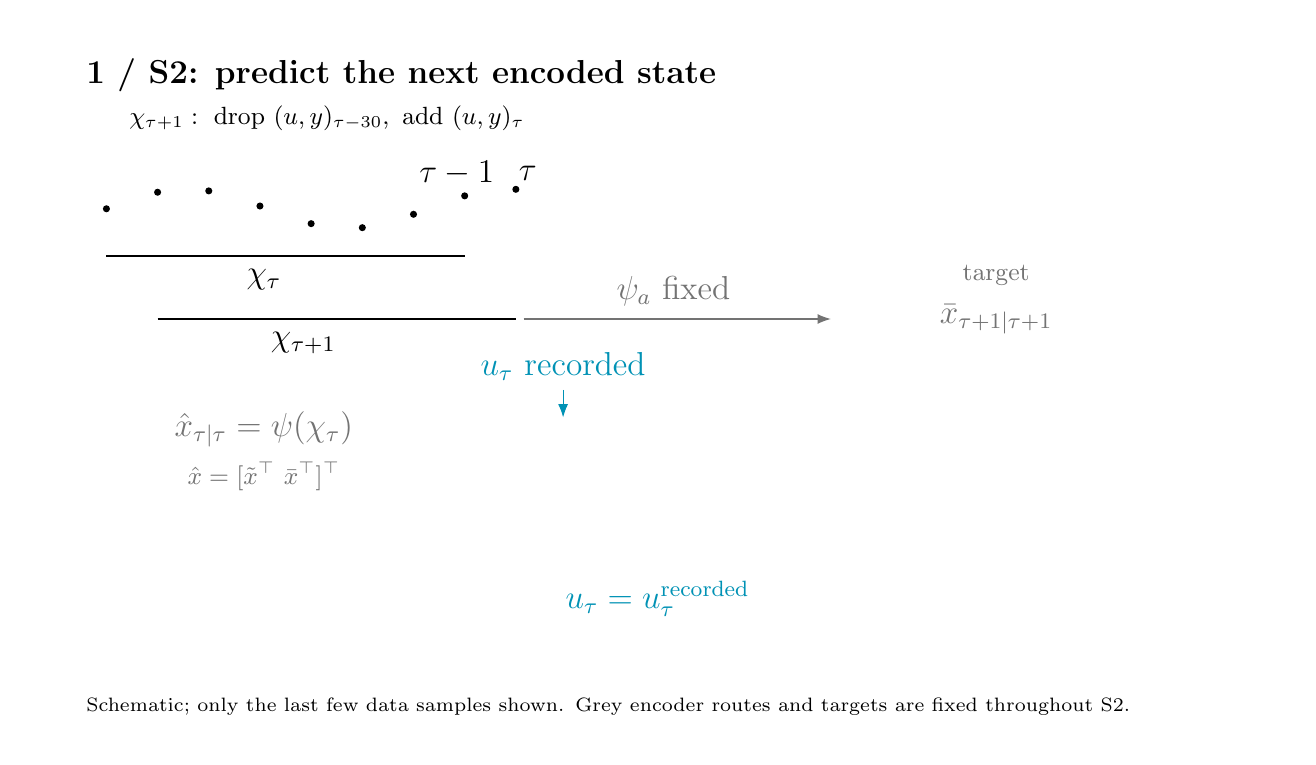
\begin{tikzpicture}\useasboundingbox (0,0) rectangle (16,9);\fill[white] (0,0) rectangle (16,9);\fontsize{12}{14}\selectfont
\node[anchor=west,font=\large\bfseries] at (0.6,8.4) {1 / S2: predict the next encoded state};
\node[anchor=west,font=\scriptsize,text width=14.8cm,align=left] at (0.6,0.38) {Schematic; only the last few data samples shown. Grey encoder routes and targets are fixed throughout S2.};
\fill (1.0,6.700) circle (.045);
\fill (1.65,6.910) circle (.045);
\fill (2.3,6.927) circle (.045);
\fill (2.95,6.735) circle (.045);
\fill (3.6,6.511) circle (.045);
\fill (4.25,6.460) circle (.045);
\fill (4.9,6.630) circle (.045);
\fill (5.55,6.864) circle (.045);
\fill (6.2,6.947) circle (.045);
\node[] at (5.45,7.15) {$\tau-1$};
\node[] at (6.35,7.15) {$\tau$};
\draw[black] (1,6.1) -- (5.55,6.1);
\node[] at (3,5.8) {$\chi_\tau$};
\draw[black] (1.65,5.3) -- (6.2,5.3);
\node[black] at (3.5,5) {$\chi_{\tau+1}$};
\node[black,font=\small] at (3.8,7.85) {$\chi_{\tau+1}:\ \text{drop }(u,y)_{\tau-30},\ \text{add }(u,y)_\tau$};
\draw[->,black!55] (6.3,5.3) -- (10.2,5.3);
\node[black!55] at (8.2,5.65) {$\psi_a$ fixed};
\node[black!55] at (12.3,5.3) {$\bar x_{\tau+1|\tau+1}$};
\node[font=\small,black!55] at (12.3,5.85) {target};
\node[black!55] at (3,3.9) {$\hat x_{\tau|\tau}=\psi(\chi_\tau)$};
\node[font=\small,black!55] at (3,3.3) {$\hat x=[\tilde x^\top\ \bar x^\top]^\top$};
\node[hl] at (6.8,4.7) {$u_\tau$ recorded};
\draw[->,hl] (6.8,4.4) -- (6.8,4.05);
\node[hl] at (8,1.75) {$u_\tau=u_\tau^{\rm recorded}$};
\end{tikzpicture}
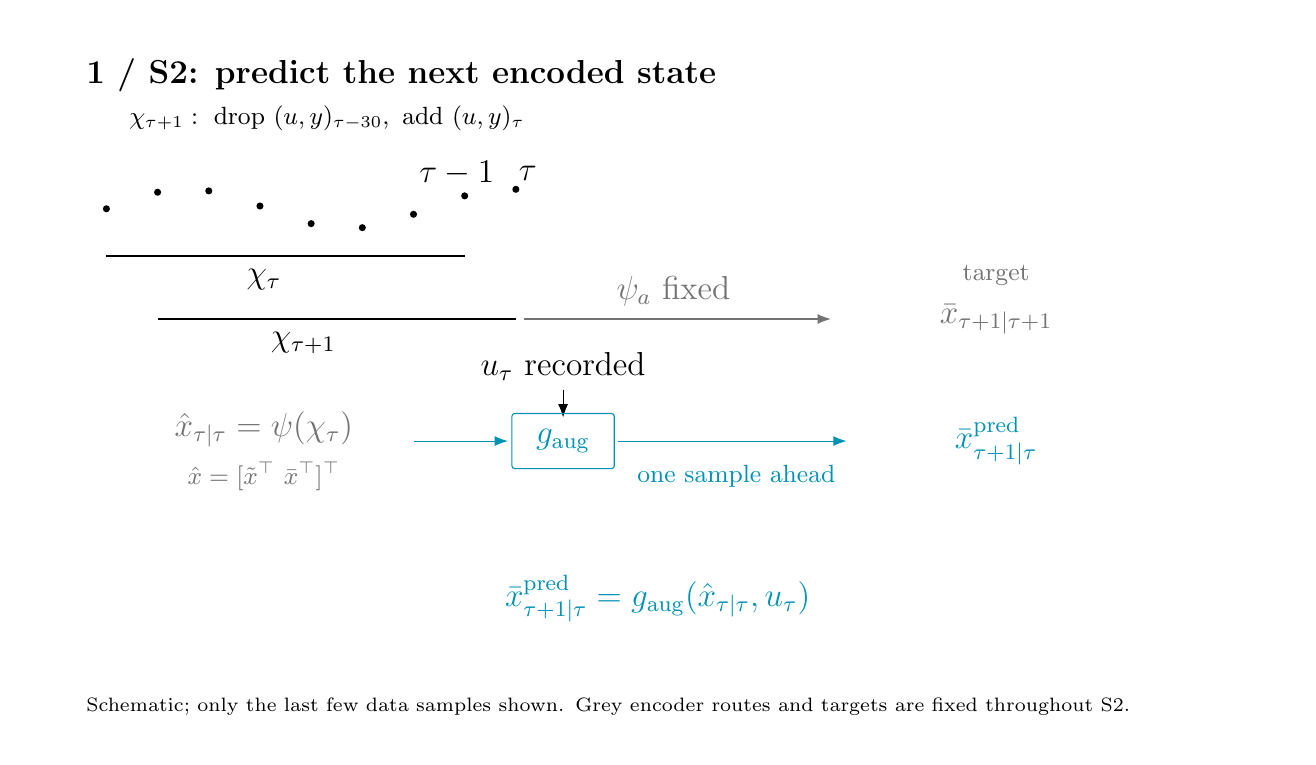
\begin{tikzpicture}\useasboundingbox (0,0) rectangle (16,9);\fill[white] (0,0) rectangle (16,9);\fontsize{12}{14}\selectfont
\node[anchor=west,font=\large\bfseries] at (0.6,8.4) {1 / S2: predict the next encoded state};
\node[anchor=west,font=\scriptsize,text width=14.8cm,align=left] at (0.6,0.38) {Schematic; only the last few data samples shown. Grey encoder routes and targets are fixed throughout S2.};
\fill (1.0,6.700) circle (.045);
\fill (1.65,6.910) circle (.045);
\fill (2.3,6.927) circle (.045);
\fill (2.95,6.735) circle (.045);
\fill (3.6,6.511) circle (.045);
\fill (4.25,6.460) circle (.045);
\fill (4.9,6.630) circle (.045);
\fill (5.55,6.864) circle (.045);
\fill (6.2,6.947) circle (.045);
\node[] at (5.45,7.15) {$\tau-1$};
\node[] at (6.35,7.15) {$\tau$};
\draw[black] (1,6.1) -- (5.55,6.1);
\node[] at (3,5.8) {$\chi_\tau$};
\draw[black] (1.65,5.3) -- (6.2,5.3);
\node[black] at (3.5,5) {$\chi_{\tau+1}$};
\node[black,font=\small] at (3.8,7.85) {$\chi_{\tau+1}:\ \text{drop }(u,y)_{\tau-30},\ \text{add }(u,y)_\tau$};
\draw[->,black!55] (6.3,5.3) -- (10.2,5.3);
\node[black!55] at (8.2,5.65) {$\psi_a$ fixed};
\node[black!55] at (12.3,5.3) {$\bar x_{\tau+1|\tau+1}$};
\node[font=\small,black!55] at (12.3,5.85) {target};
\node[black!55] at (3,3.9) {$\hat x_{\tau|\tau}=\psi(\chi_\tau)$};
\node[font=\small,black!55] at (3,3.3) {$\hat x=[\tilde x^\top\ \bar x^\top]^\top$};
\node[black] at (6.8,4.7) {$u_\tau$ recorded};
\draw[->,black] (6.8,4.4) -- (6.8,4.05);
\node[blk,hl] at (6.8,3.75) {$g_{\rm aug}$};
\draw[->,hl] (4.9,3.75) -- (6.1,3.75);
\draw[->,hl] (7.5,3.75) -- (10.4,3.75);
\node[hl] at (12.3,3.75) {$\bar x_{\tau+1|\tau}^{\rm pred}$};
\node[font=\small,hl] at (9,3.3) {one sample ahead};
\node[hl] at (8,1.75) {$\bar x^{\rm pred}_{\tau+1|\tau}=g_{\rm aug}(\hat x_{\tau|\tau},u_\tau)$};
\end{tikzpicture}
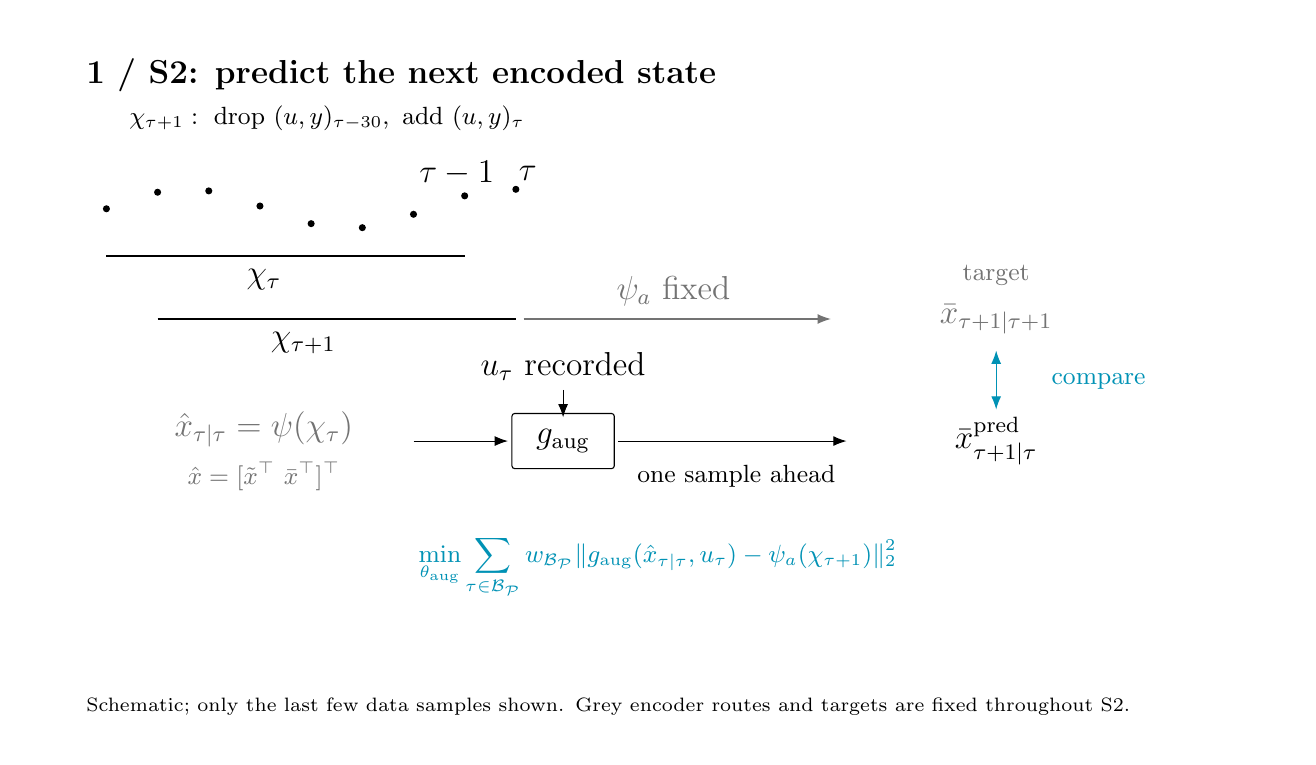
\begin{tikzpicture}\useasboundingbox (0,0) rectangle (16,9);\fill[white] (0,0) rectangle (16,9);\fontsize{12}{14}\selectfont
\node[anchor=west,font=\large\bfseries] at (0.6,8.4) {1 / S2: predict the next encoded state};
\node[anchor=west,font=\scriptsize,text width=14.8cm,align=left] at (0.6,0.38) {Schematic; only the last few data samples shown. Grey encoder routes and targets are fixed throughout S2.};
\fill (1.0,6.700) circle (.045);
\fill (1.65,6.910) circle (.045);
\fill (2.3,6.927) circle (.045);
\fill (2.95,6.735) circle (.045);
\fill (3.6,6.511) circle (.045);
\fill (4.25,6.460) circle (.045);
\fill (4.9,6.630) circle (.045);
\fill (5.55,6.864) circle (.045);
\fill (6.2,6.947) circle (.045);
\node[] at (5.45,7.15) {$\tau-1$};
\node[] at (6.35,7.15) {$\tau$};
\draw[black] (1,6.1) -- (5.55,6.1);
\node[] at (3,5.8) {$\chi_\tau$};
\draw[black] (1.65,5.3) -- (6.2,5.3);
\node[black] at (3.5,5) {$\chi_{\tau+1}$};
\node[black,font=\small] at (3.8,7.85) {$\chi_{\tau+1}:\ \text{drop }(u,y)_{\tau-30},\ \text{add }(u,y)_\tau$};
\draw[->,black!55] (6.3,5.3) -- (10.2,5.3);
\node[black!55] at (8.2,5.65) {$\psi_a$ fixed};
\node[black!55] at (12.3,5.3) {$\bar x_{\tau+1|\tau+1}$};
\node[font=\small,black!55] at (12.3,5.85) {target};
\node[black!55] at (3,3.9) {$\hat x_{\tau|\tau}=\psi(\chi_\tau)$};
\node[font=\small,black!55] at (3,3.3) {$\hat x=[\tilde x^\top\ \bar x^\top]^\top$};
\node[black] at (6.8,4.7) {$u_\tau$ recorded};
\draw[->,black] (6.8,4.4) -- (6.8,4.05);
\node[blk,black] at (6.8,3.75) {$g_{\rm aug}$};
\draw[->,black] (4.9,3.75) -- (6.1,3.75);
\draw[->,black] (7.5,3.75) -- (10.4,3.75);
\node[black] at (12.3,3.75) {$\bar x_{\tau+1|\tau}^{\rm pred}$};
\node[font=\small,black] at (9,3.3) {one sample ahead};
\draw[<->,hl] (12.3,4.15) -- (12.3,4.9);
\node[font=\small,hl] at (13.6,4.5) {compare};
\node[hl,font=\small] at (8,2.15) {$\displaystyle\min_{\theta_{\rm aug}}\sum_{\tau\in\mathcal B_{\mathcal P}}w_{\mathcal B_{\mathcal P}}\|g_{\rm aug}(\hat x_{\tau|\tau},u_\tau)-\psi_a(\chi_{\tau+1})\|_2^2$};
\end{tikzpicture}
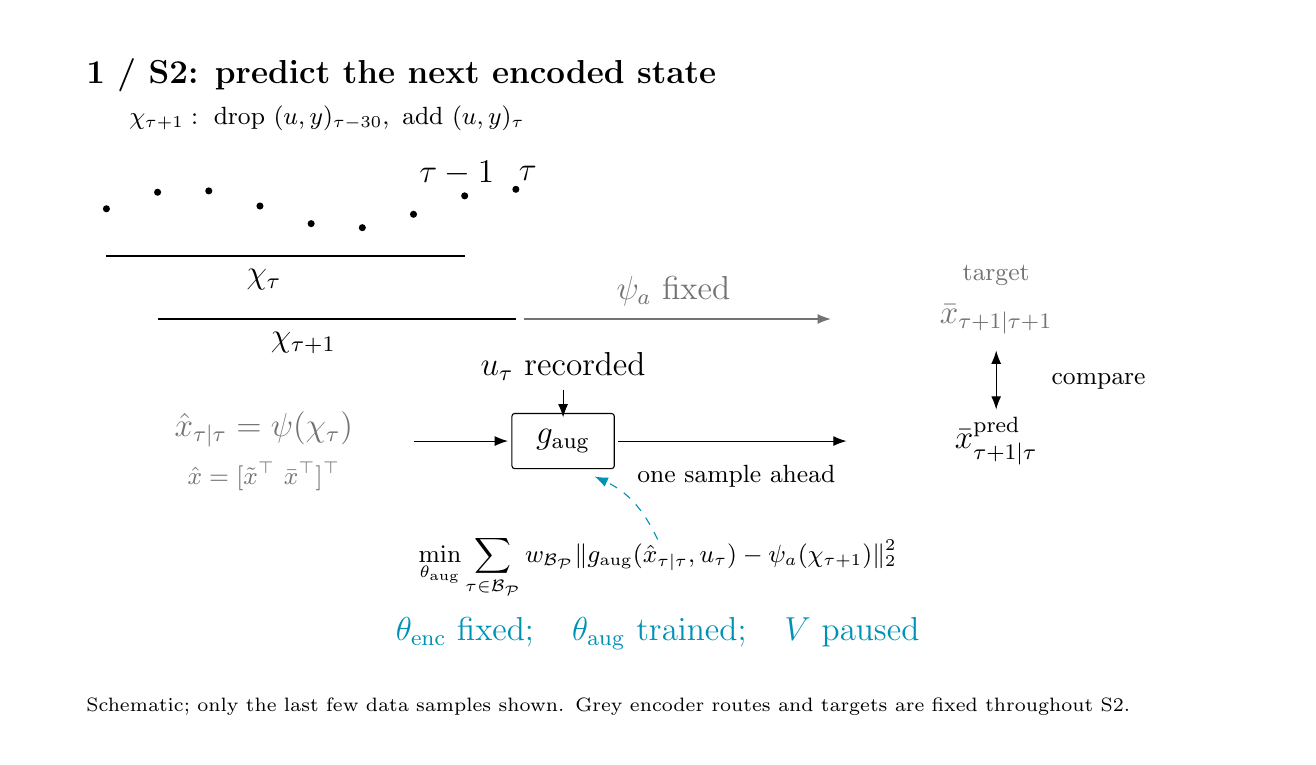
\begin{tikzpicture}\useasboundingbox (0,0) rectangle (16,9);\fill[white] (0,0) rectangle (16,9);\fontsize{12}{14}\selectfont
\node[anchor=west,font=\large\bfseries] at (0.6,8.4) {1 / S2: predict the next encoded state};
\node[anchor=west,font=\scriptsize,text width=14.8cm,align=left] at (0.6,0.38) {Schematic; only the last few data samples shown. Grey encoder routes and targets are fixed throughout S2.};
\fill (1.0,6.700) circle (.045);
\fill (1.65,6.910) circle (.045);
\fill (2.3,6.927) circle (.045);
\fill (2.95,6.735) circle (.045);
\fill (3.6,6.511) circle (.045);
\fill (4.25,6.460) circle (.045);
\fill (4.9,6.630) circle (.045);
\fill (5.55,6.864) circle (.045);
\fill (6.2,6.947) circle (.045);
\node[] at (5.45,7.15) {$\tau-1$};
\node[] at (6.35,7.15) {$\tau$};
\draw[black] (1,6.1) -- (5.55,6.1);
\node[] at (3,5.8) {$\chi_\tau$};
\draw[black] (1.65,5.3) -- (6.2,5.3);
\node[black] at (3.5,5) {$\chi_{\tau+1}$};
\node[black,font=\small] at (3.8,7.85) {$\chi_{\tau+1}:\ \text{drop }(u,y)_{\tau-30},\ \text{add }(u,y)_\tau$};
\draw[->,black!55] (6.3,5.3) -- (10.2,5.3);
\node[black!55] at (8.2,5.65) {$\psi_a$ fixed};
\node[black!55] at (12.3,5.3) {$\bar x_{\tau+1|\tau+1}$};
\node[font=\small,black!55] at (12.3,5.85) {target};
\node[black!55] at (3,3.9) {$\hat x_{\tau|\tau}=\psi(\chi_\tau)$};
\node[font=\small,black!55] at (3,3.3) {$\hat x=[\tilde x^\top\ \bar x^\top]^\top$};
\node[black] at (6.8,4.7) {$u_\tau$ recorded};
\draw[->,black] (6.8,4.4) -- (6.8,4.05);
\node[blk,black] at (6.8,3.75) {$g_{\rm aug}$};
\draw[->,black] (4.9,3.75) -- (6.1,3.75);
\draw[->,black] (7.5,3.75) -- (10.4,3.75);
\node[black] at (12.3,3.75) {$\bar x_{\tau+1|\tau}^{\rm pred}$};
\node[font=\small,black] at (9,3.3) {one sample ahead};
\draw[<->,black] (12.3,4.15) -- (12.3,4.9);
\node[font=\small,black] at (13.6,4.5) {compare};
\node[black,font=\small] at (8,2.15) {$\displaystyle\min_{\theta_{\rm aug}}\sum_{\tau\in\mathcal B_{\mathcal P}}w_{\mathcal B_{\mathcal P}}\|g_{\rm aug}(\hat x_{\tau|\tau},u_\tau)-\psi_a(\chi_{\tau+1})\|_2^2$};
\node[hl] at (8,1.3) {$\theta_{\rm enc}\ \text{fixed};\quad \theta_{\rm aug}\ \text{trained};\quad V\ \text{paused}$};
\draw[->,hl,dashed] (8,2.5) to[bend right=20] (7.2,3.3);
\end{tikzpicture}
\end{document}